\documentclass[14Q,twocolumn]{jsarticle}
\usepackage[dvipdfmx]{graphicx}
\usepackage{wrapfig}
\usepackage{float}
\usepackage{otf}
\usepackage{longtable}
\usepackage{ulem}
\usepackage{ascmac}
\usepackage{multicol}
%%%%%
\makeatletter
\newenvironment{tablehere}
  {\def\@captype{table}}
  {}
\newenvironment{figurehere}
  {\def\@captype{figure}}
  {}
\makeatother
%%%%%%
\setlength{\textwidth}{160truemm}      % テキスト幅: 160mm
\setlength{\fullwidth}{\textwidth}     % ページ全体の幅
\setlength{\oddsidemargin}{0mm}   % 左余白
\setlength{\topmargin}{-10mm}       % 上余白
\setlength{\textheight}{240truemm}     % テキスト高さ: 297-(30+30)=237mm
\pagestyle{empty}
\title{QGISで遺跡立地分析}% 文書のタイトル
\date{2018年9月18日}
\author{厚沢部町 石 井 淳 平}              % 著者

%------------------------------
\begin{document}
\maketitle
%\begin{multicols}{2}
\section{この時間に覚えること}
プロセッシング機能を利用してGRASS GISの分析機能を使用します。GRASS GISの豊富な機能の中から傾斜や傾斜方位の他に日射量の算出を行います。QGISに用意されている豊富なプラグインのインストール方法を学びながら「Point sampling tool」プラグインを利用して地形データの取得を行います。

以上のようにして取得した地形データから遺跡の立地条件を検討します。

\begin{itemize}
\item 標高データから新たな地形指標を作成する
\item プロセッシング機能を使った他のGISソフト機能の利用
\item プラグインを使う
\item PointSamplingtoolを使用した地形データの取得
\item GISデータを利用した統計処理
\end{itemize}


%%%%
\section{プロセッシング機能とは}

\begin{itemize}
\item とても高機能なGRASS GISの機能を使う
\item GRASS GISで傾斜方位と傾斜角度、日射量を計算する
\item GRASS GISのほかにもSAGA GISなどマニアックな機能をQGISから利用できる
\item 一つ一つのGISソフトウェアの作法を覚えなくてもよい
\end{itemize}


%%%%
\section{プロセッシング機能を有効化する}
プロセッシング機能を使うためには使用するソフトウェアを有効にする必要があります。

\begin{enumerate}
\item 「プロセッシング」→「ツールボックス」
\item 「オプション」をクリック
\item 「プロバイダ」→「GRASS」→「有効化」にチェック
\end{enumerate}

\begin{figurehere}
\centering
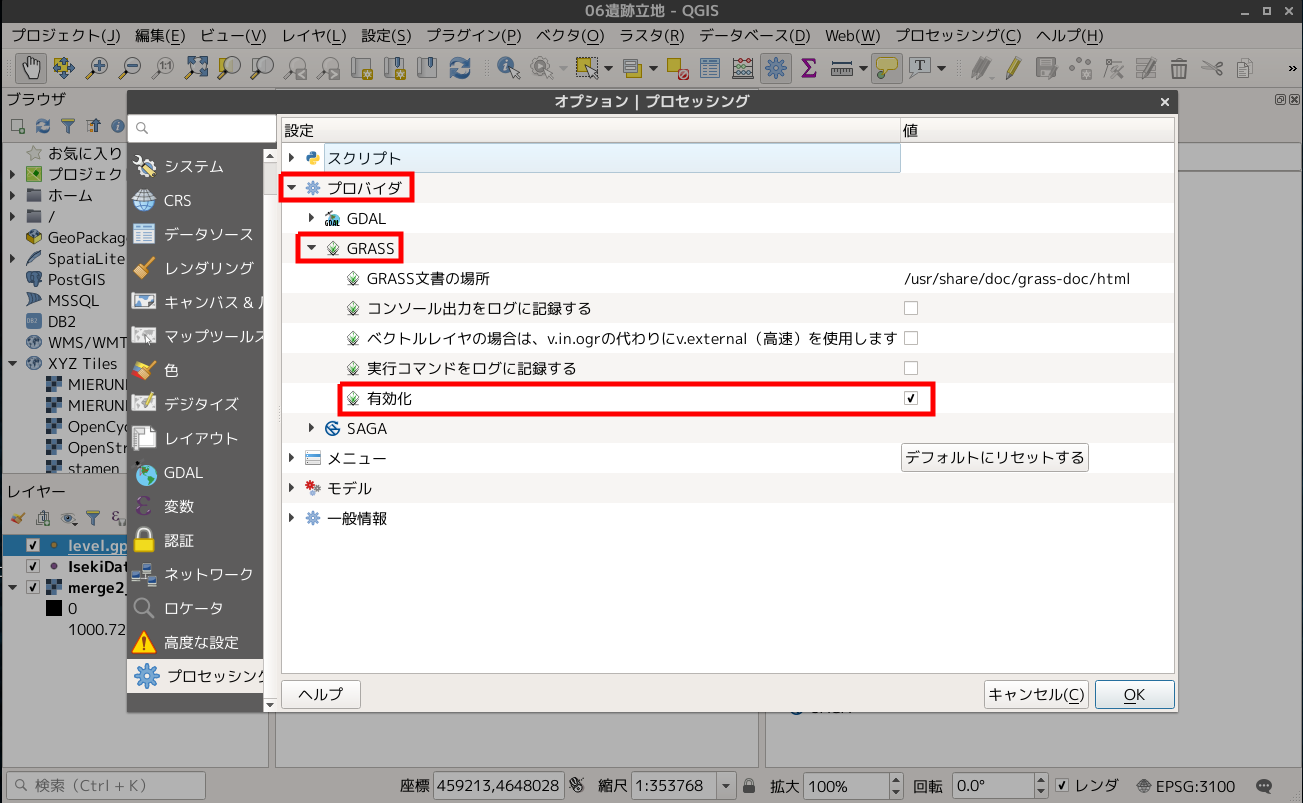
\includegraphics[width=1\linewidth]{10.png}
\caption{プロセッシングツールボックスを開いてGRASS GISを有効にする}
\end{figurehere}


%%%%
\section{傾斜角度と傾斜方位を算出する}
GRASS GISの「r.slope.aspect」コマンドを使って傾斜角度と傾斜方位を算出します。

\begin{enumerate}
\item 「GRASS」→「Raster」→「r.slope.aspect」
\item 「Elevation」には「merge2utm54」(標高)を指定
\item 「Slope」と「Aspect」のチェックボックスにチェック
\item  保存ファイル名は「slope」と「aspect」
\end{enumerate}

\begin{figurehere}
\centering
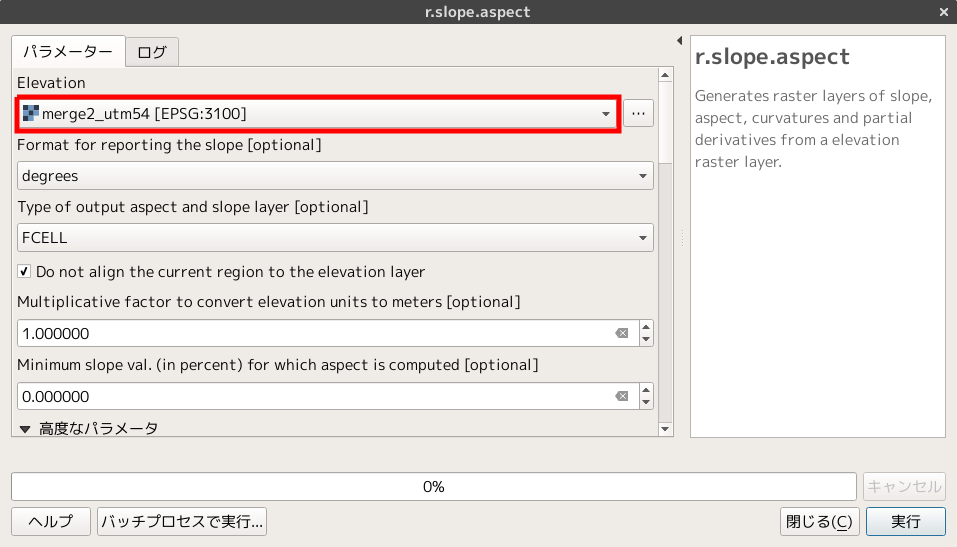
\includegraphics[width=1\linewidth]{12.png}
\caption{入力する標高データを指定}
\end{figurehere}

\begin{figurehere}
\centering
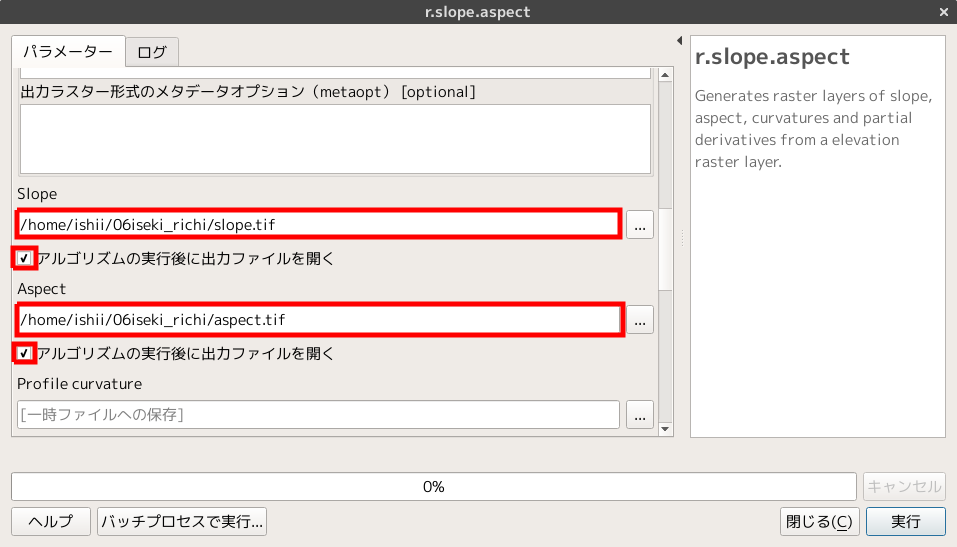
\includegraphics[width=1\linewidth]{13.png}
\caption{保存ファイル名をを指定}
\end{figurehere}

\begin{figurehere}
\centering
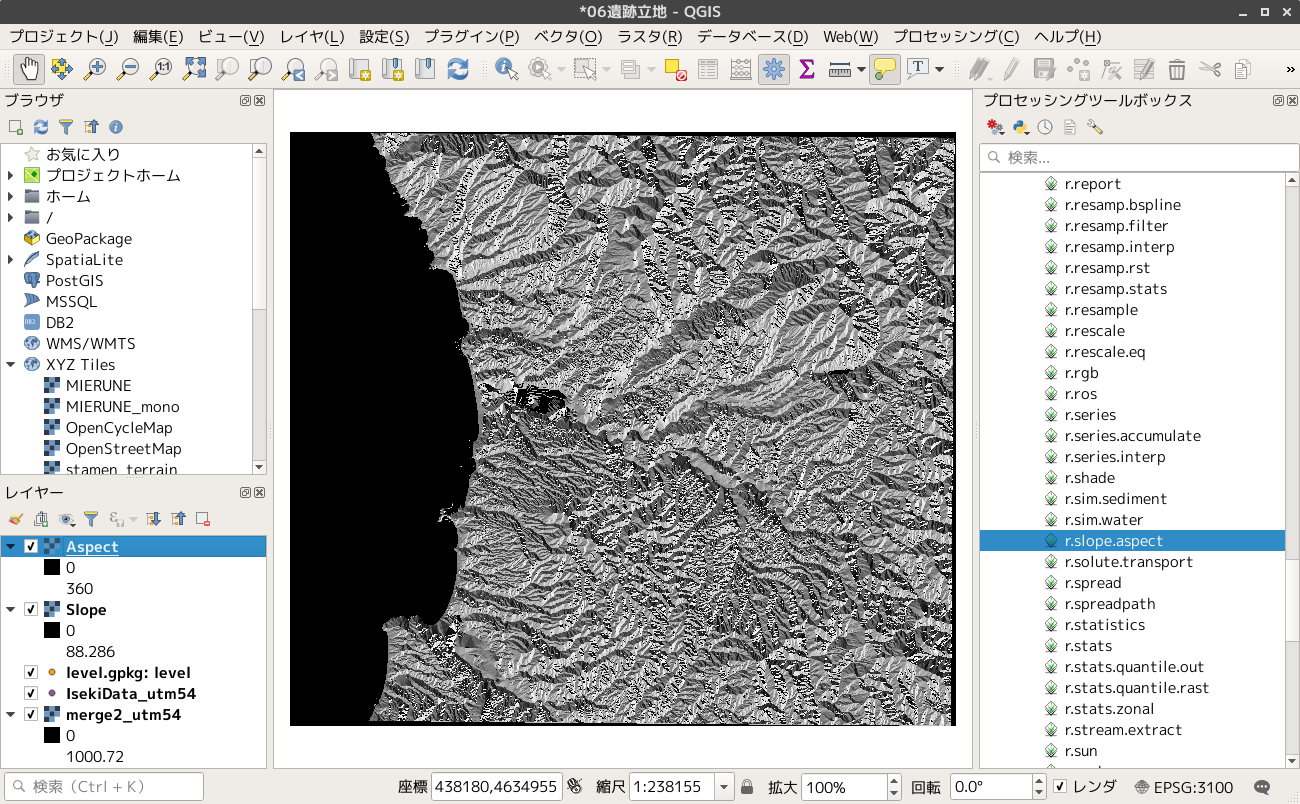
\includegraphics[width=1\linewidth]{14.png}
\caption{傾斜方位ラスタ}
\end{figurehere}

\begin{figurehere}
\centering
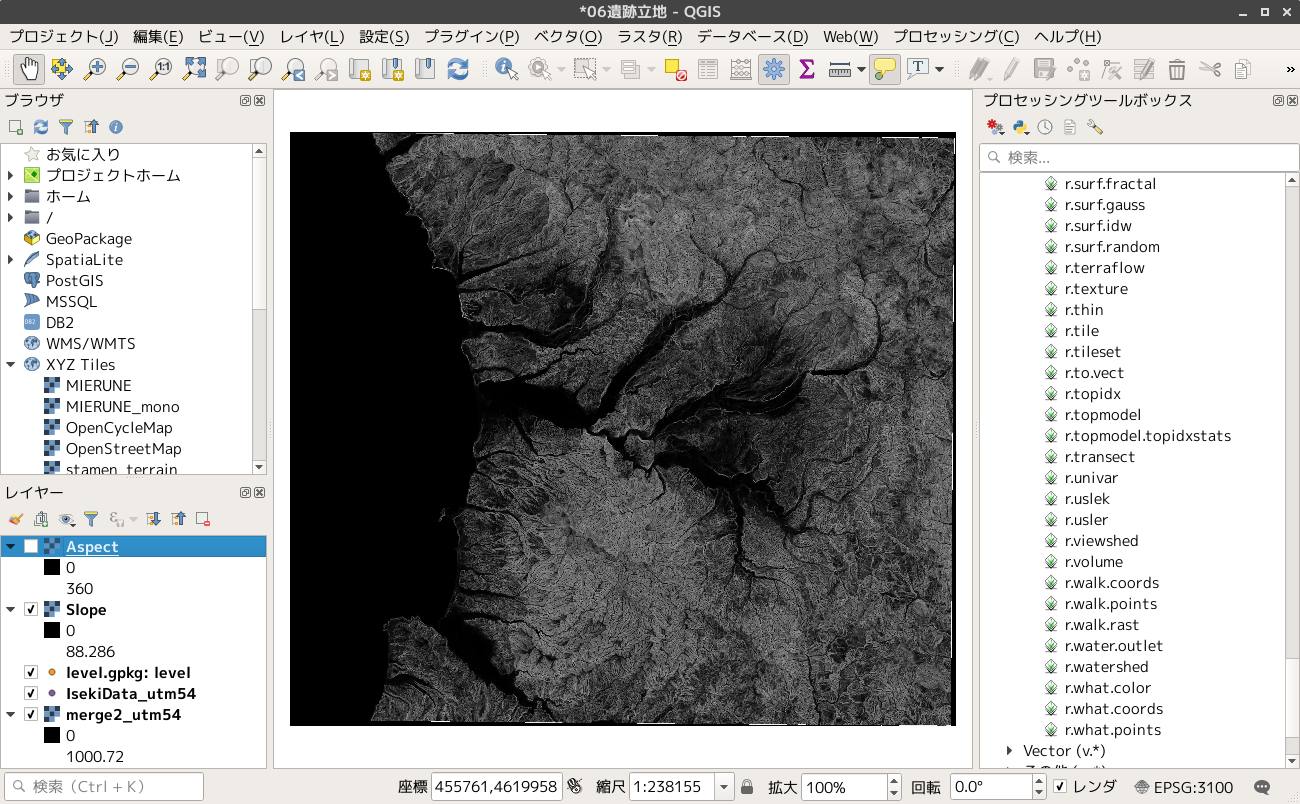
\includegraphics[width=1\linewidth]{15.png}
\caption{傾斜角度ラスタ}
\end{figurehere}

%%%%
\section{GRASS GISの傾斜方位の注意点}
GRASS GISの傾斜方位にはトラップとも呼べる注意点があります。東が原点であること、角度は半時計回りだということを覚えておかないと悲惨なことになります。

\begin{itemize}
\item 原点は東
\item 角度は半時計回り
\item  東向きの斜面が0度、北向きの斜面は90度、西は180度、南は270度
\end{itemize}


%%%%
\section{日射量を算出する}
GRASS GISの「r.sun」コマンドを使用します。

\begin{enumerate}
\item 「Elevation layer」→「merg2utm54」
\item 「Aspect layer」→「Aspect」
\item 「A single value...」→「270」(傾斜方位の「南」の値を指定)
\item 「name of the input raster map」→「Slope」
\end{enumerate}

\begin{figurehere}
\centering
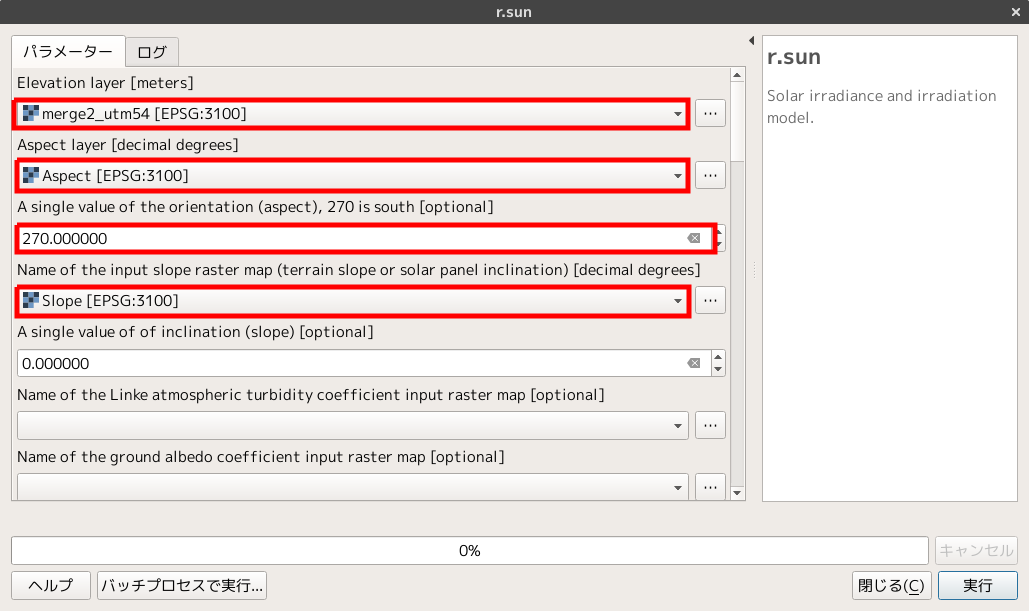
\includegraphics[width=1\linewidth]{18.png}
\caption{r.sunコマンドの設定その1}
\end{figurehere}


\begin{enumerate}
\item 「No. of day of the year」(1月1日を基点にした日数)→「173」(夏至の頃を指定) 
\item 「Global(total) irradiance」(合計放射輝度)にチェック
\item  ファイル名「irradiation」
\item 「Global(total) irradiance」(合計放射輝度)にチェック
\item ファイル名「irradiation」
\end{enumerate}

\begin{figurehere}
\centering
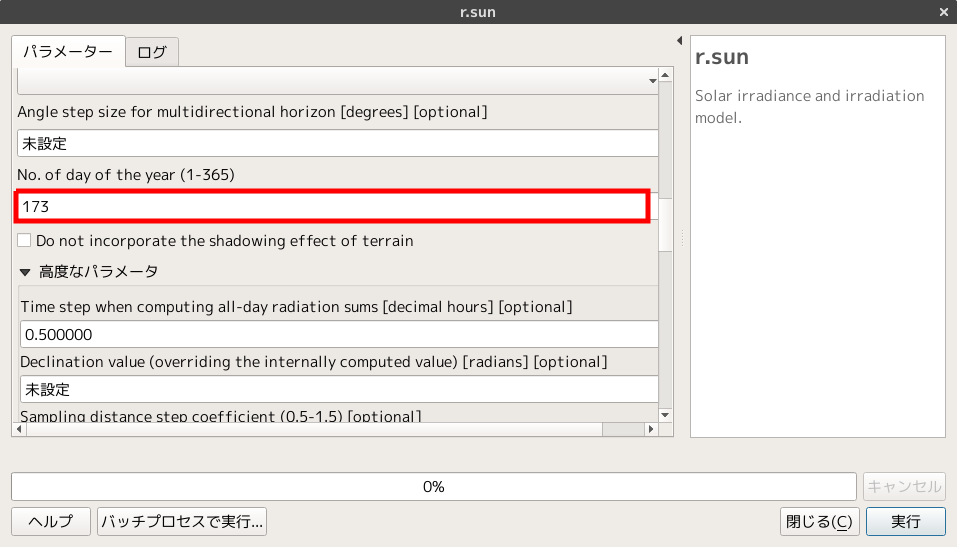
\includegraphics[width=1\linewidth]{19.png}
\caption{r.sunコマンドの設定その2}
\end{figurehere}

\begin{figurehere}
\centering
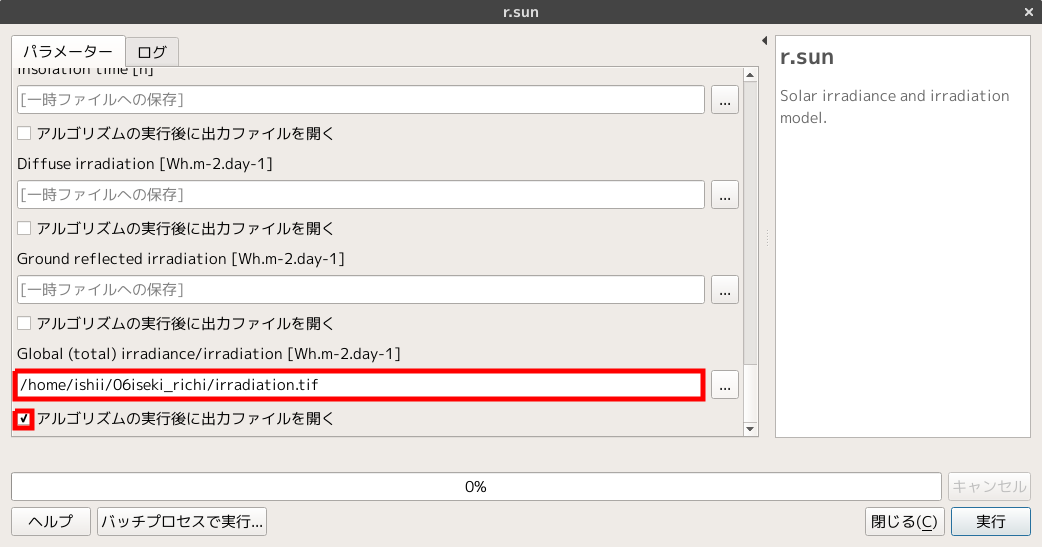
\includegraphics[width=1\linewidth]{20.png}
\caption{r.sunコマンドの設定その3}
\end{figurehere}

\begin{figurehere}
\centering
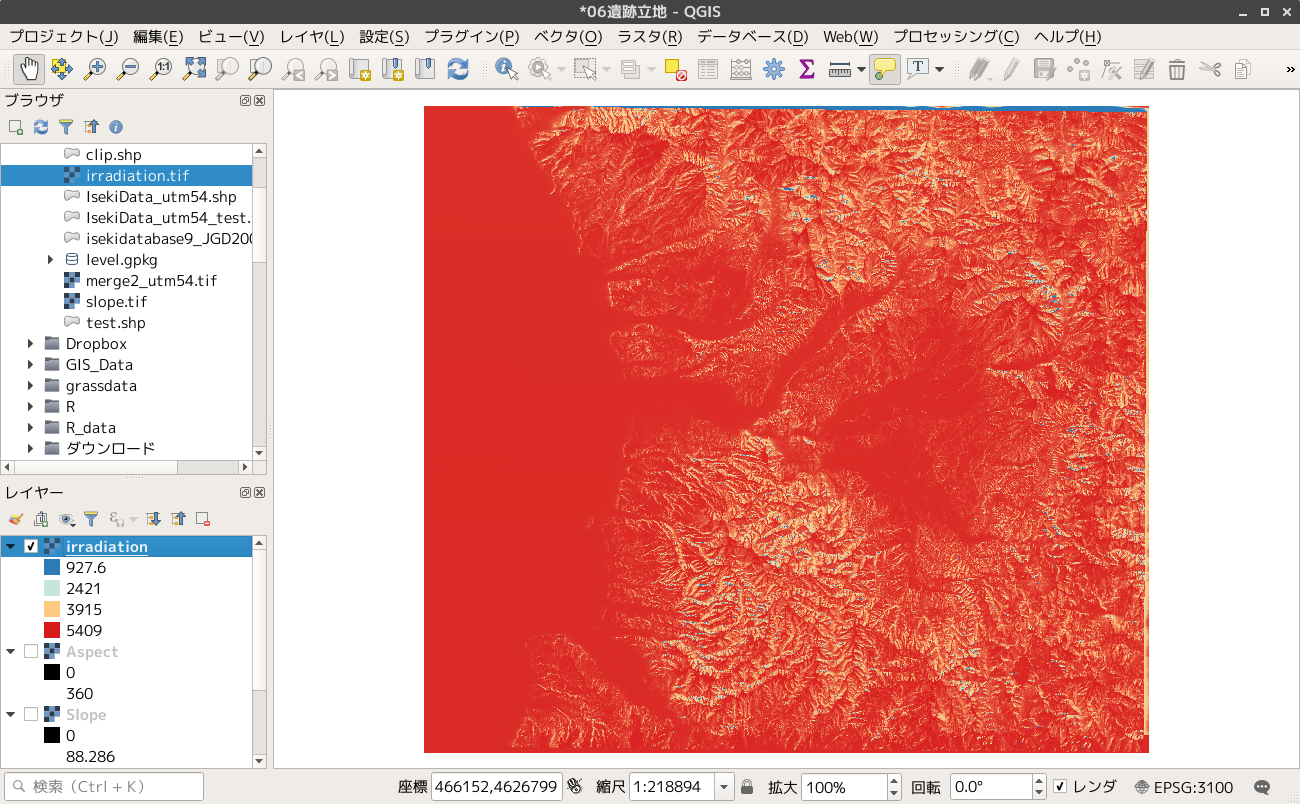
\includegraphics[width=1\linewidth]{22.png}
\caption{日射量ラスタ}
\end{figurehere}

%%%%
\section{河川データについて}
\begin{itemize}
\item 国土地理院基盤地図情報
	\begin{itemize}
	\item 主要な河川を網羅
	\item ラインデータとポリゴン(内水面)の2種
	\end{itemize}
\item 国土交通省国土基本情報
	\begin{itemize}
	\item ラインデータのみ
	\item 小河川まで網羅
	\end{itemize}
\end{itemize}

%%%%
\section{河川データのラスタ化}
遺跡の立地に関係しそうな要素として河川からの距離が考えられます。遺跡の立地地点から河川までの距離を算出する方法はたくさんありますが、ここでは河川からの距離をラスタ地図化して使用します。ラスタ化するメリットは遺跡データの増減があっても容易に対応可能であることやラスタ計算を行う上で有利となるからです。

\begin{enumerate}
\item 「ラスタ」→「変換」→「ベクタ化(ラスタのベクタ化)」
\item 「入力レイヤ」→「kokudoWLutm54」(河川ラインデータ)
\item 「A fixed value to burn」(データのあるところに入力する値)→1.0
\item 「出力ラスターサイズの単位」→「Georeferenced units」(投影系上の単位 ここではm)
\item 「幅/水平方向の解像度」→10
\item 「出力領域」(ラスタ化する領域の端点を入力)→417000.0 459000.0 4621000.0 4659000.0
\item 「出力バンドに指定されたnodata値を割り当てる」(データのないところに入力する値)→0
\item 「ラスタ化」→WL.tif
\end{enumerate}

\begin{figurehere}
\centering
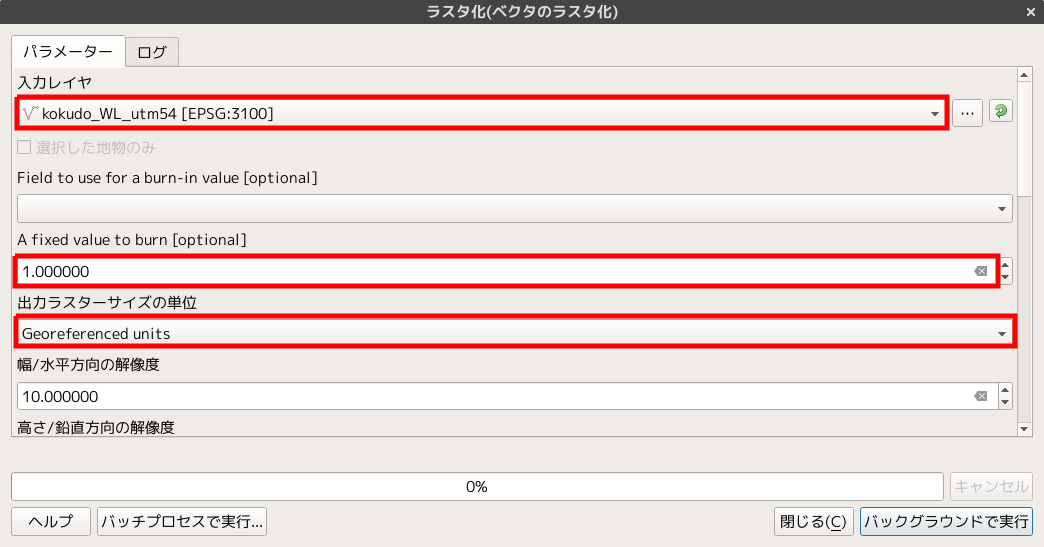
\includegraphics[width=1\linewidth]{27.png}
\caption{ラスタのベクタ化の設定その1}
\end{figurehere}

\begin{figurehere}
\centering
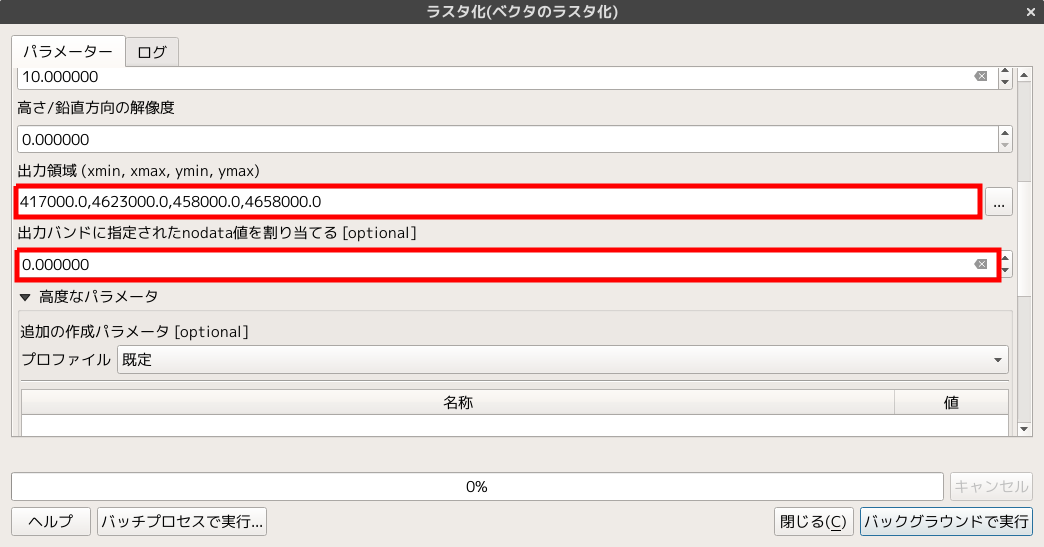
\includegraphics[width=1\linewidth]{28.png}
\caption{ラスタのベクタ化の設定その2}
\end{figurehere}

\begin{figurehere}
\centering
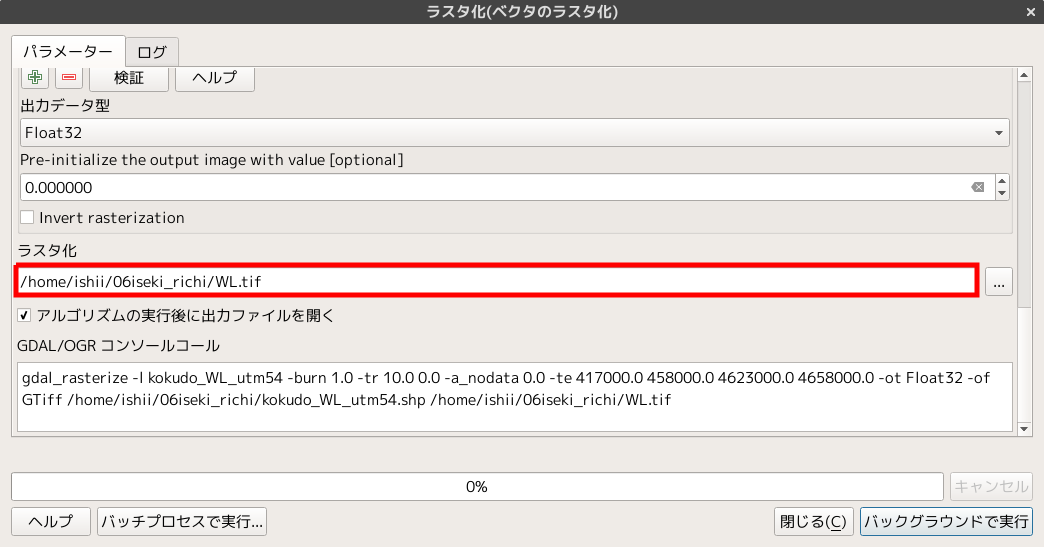
\includegraphics[width=1\linewidth]{29.png}
\caption{ラスタのベクタ化の設定その3}
\end{figurehere}

\begin{figurehere}
\centering
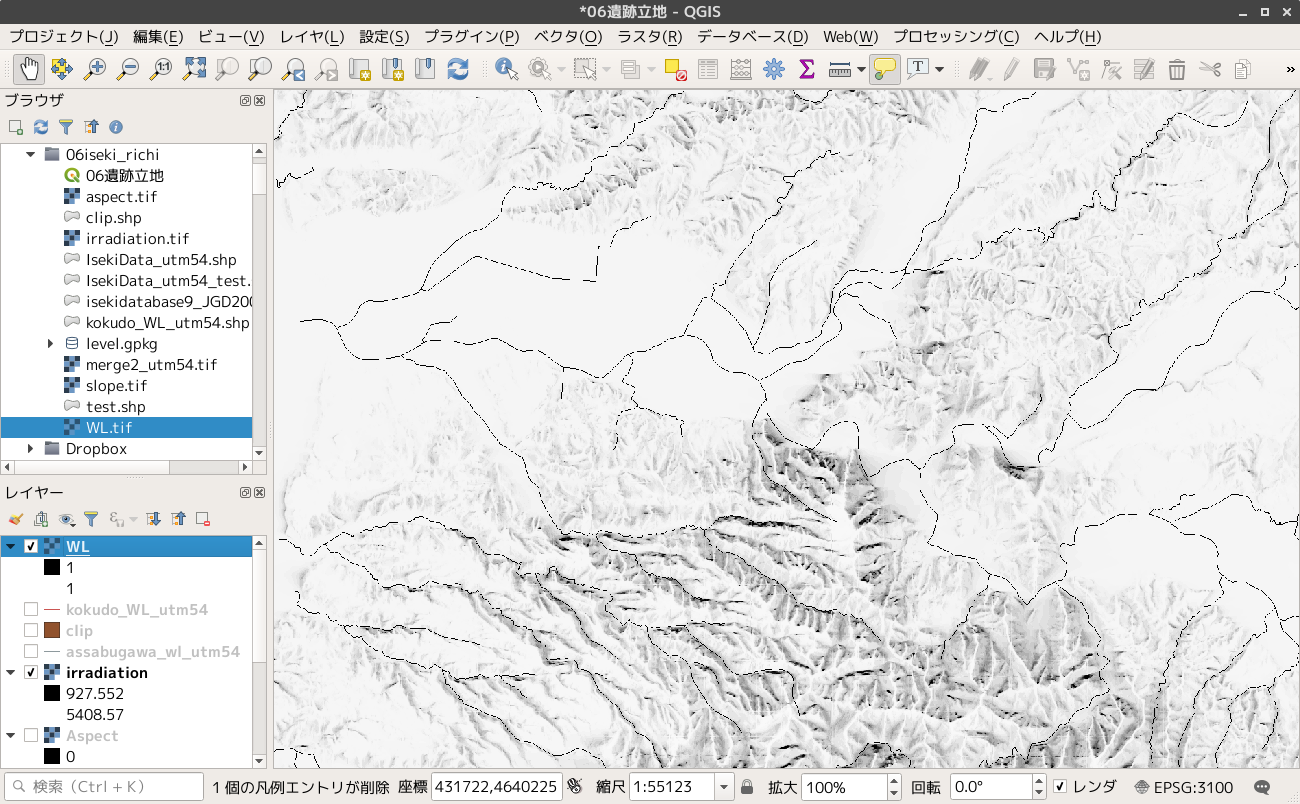
\includegraphics[width=1\linewidth]{30.png}
\caption{ラスタ化された河川データ}
\end{figurehere}

%%%%
\section{河川ラスタを距離ラスタに変換}
ラスタ化された河川データは単なる二値データです。このデータを距離ラスタに変換します。

\begin{enumerate}
\item 「ラスタ」→「解析」→「Proximity」
\item 「入力レイヤ」→「WL」(ラスタ化した河川データ)
\item 「距離単位」→「ジオリファレンス座標」(実際の距離)
\item「ファイル名」→「WLbuffer」
\end{enumerate}

\begin{figurehere}
\centering
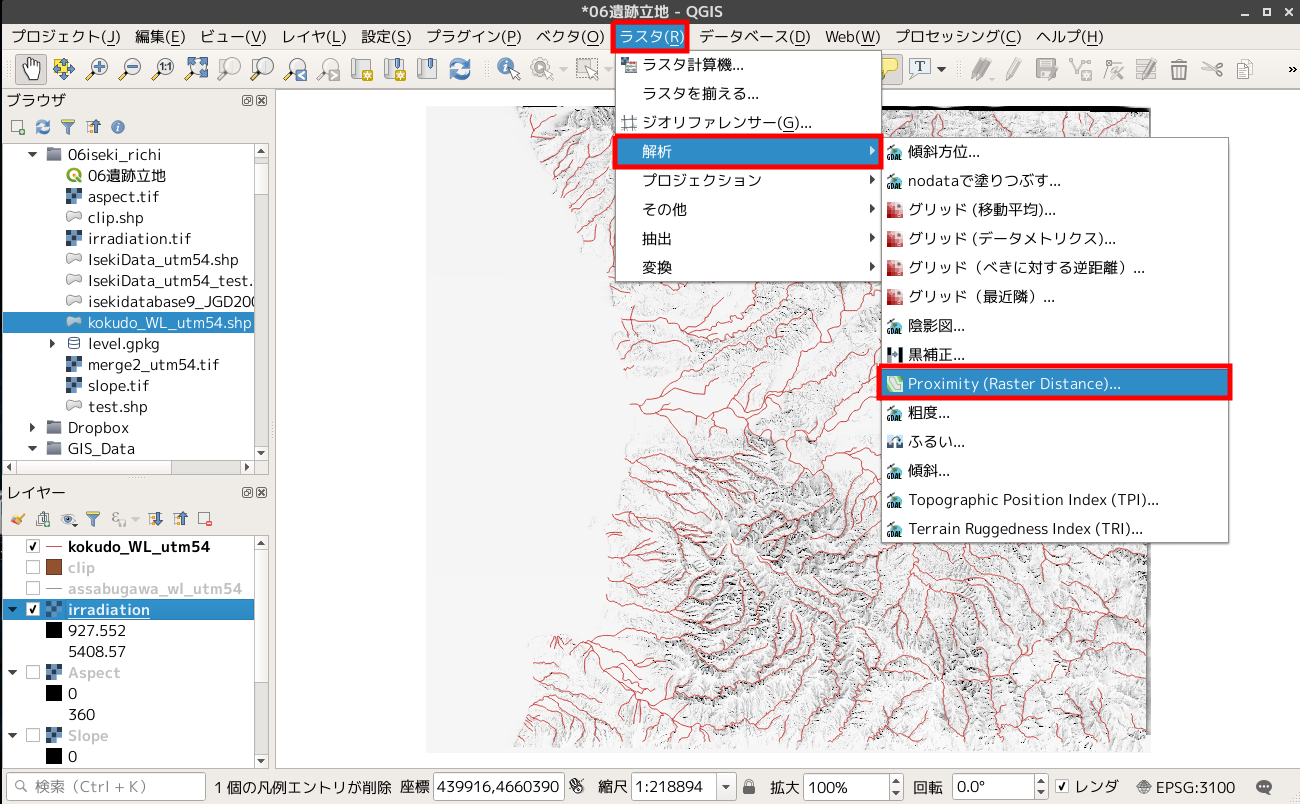
\includegraphics[width=1\linewidth]{31.png}
\caption{Proximity設定その1}
\end{figurehere}

\begin{figurehere}
\centering
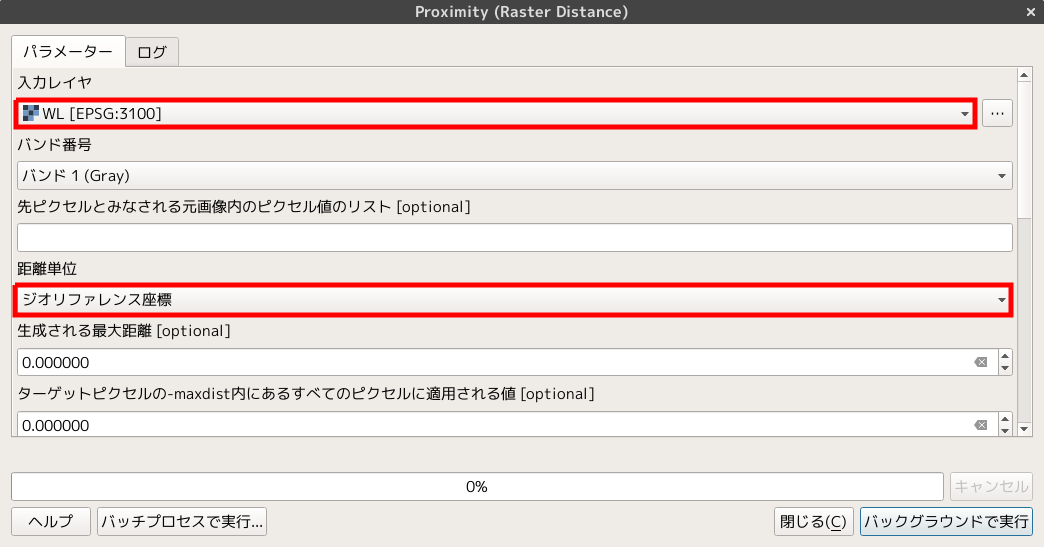
\includegraphics[width=1\linewidth]{32.png}
\caption{Proximity設定その2}
\end{figurehere}

\begin{figurehere}
\centering
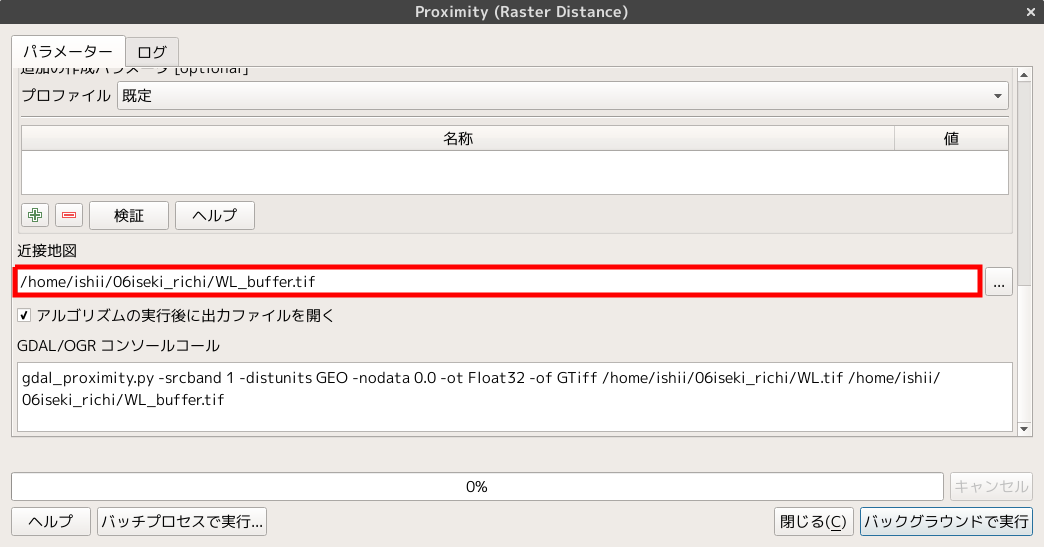
\includegraphics[width=1\linewidth]{33.png}
\caption{Proximity設定その3}
\end{figurehere}

\begin{figurehere}
\centering
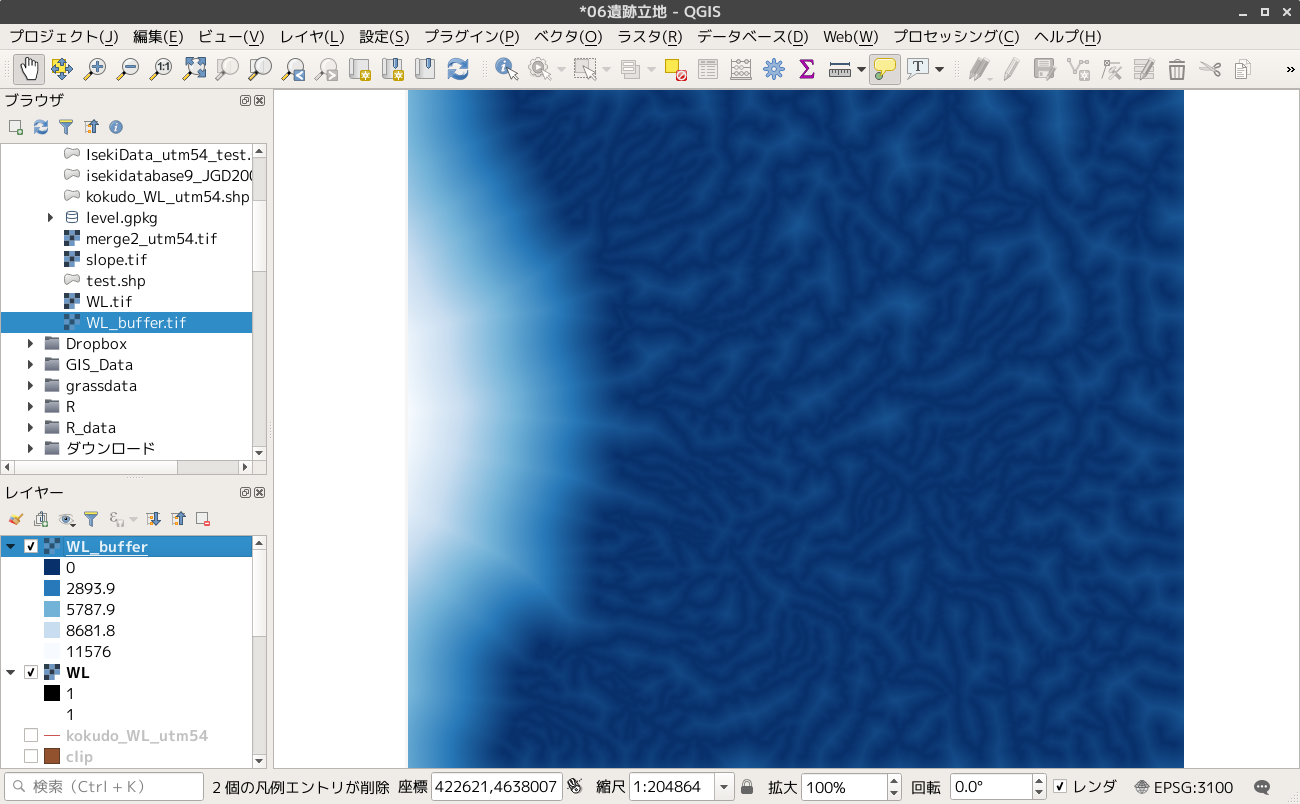
\includegraphics[width=1\linewidth]{35.png}
\caption{河川からの距離ラスタ}
\end{figurehere}

%%%%
\section{傾斜方位をカテゴリ化する}

\begin{itemize}
\item 作成した傾斜方位(Aspect.tif)は南をゼロとした連続量です。
\item このままでは統計的に扱いにくいので離散量に変換します。
\item カテゴリは「北」、「東」、「南」、「西」の4区分です。
\end{itemize}

\begin{enumerate}
\item 「ラスタ」→「ラスタ計算機」
\item 「出力レイヤ」→AspectReclass.tif
\item 「選択レイヤの領域」をクリック(Aspectレイヤを選択しておく)
\end{enumerate}

\begin{figurehere}
\centering
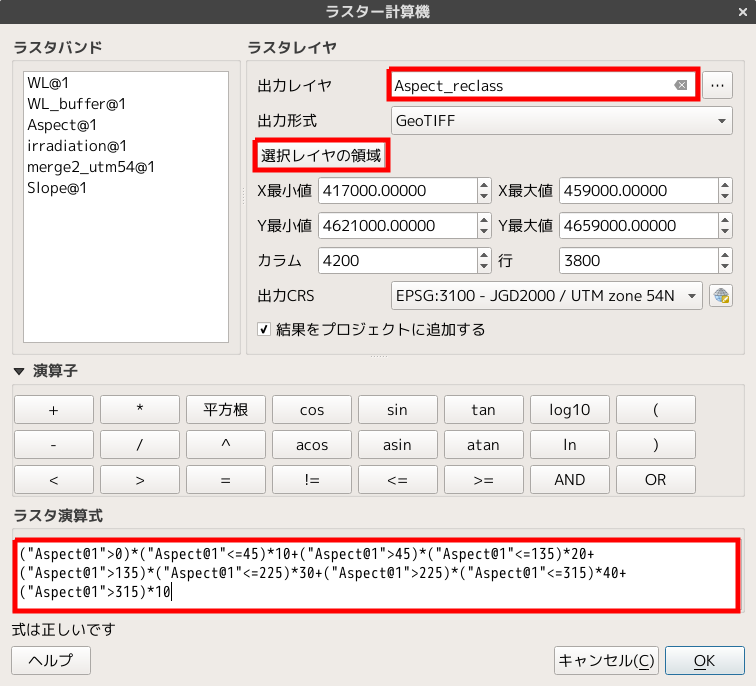
\includegraphics[width=1\linewidth]{37.png}
\caption{ラスタ計算機の設定}
\end{figurehere}

ラスタ計算機では以下のような結果を出力します。

\begin{itemize}
\item 東が0で半時計回りに増加するラスタ地図
\item 以下の式では次のような値が新たに代入される
\item 東10 北20 西30 南40
\end{itemize}

以下の計算式で方位に応じた2桁の整数値を出力します。

$
("Aspect@1">0)*("Aspect@1"<=45)*10+
("Aspect@1">45)*("Aspect@1"<=135)*20+
("Aspect@1">135)*("Aspect@1"<=225)*30+
("Aspect@1">225)*("Aspect@1"<=315)*40+
("Aspect@1">315)*10
$


\begin{enumerate}
\item $"Aspect@1"$ Aspectレイヤのバンド1を意味します。
\item $"Aspect@1">0$ 真(0より大きい)なら計算機は「1」を返し、偽なら「0」を返します。
\item $("Aspect@1">0)*("Aspect@1"<=45)$ 0より大きく45以下の値は「1」を、それ以外はすべて0が返されます。
\item $("Aspect@1">0)*("Aspect@1"<=45)*10$ 「0以上45以下」という条件を満たすピクセルには「10」が代入されます。
\item 同様に45〜135(北)では20が代入され、135〜225(西)では30が代入され、225〜315(南)では40が代入され、315〜(東)は10が代入されます。
\item (1が代入される)項は一つしかないので、全部の項を足し合わせると真となる項の数字だけが該当するピクセルに代入されます。
\end{enumerate}

\begin{figurehere}
\centering
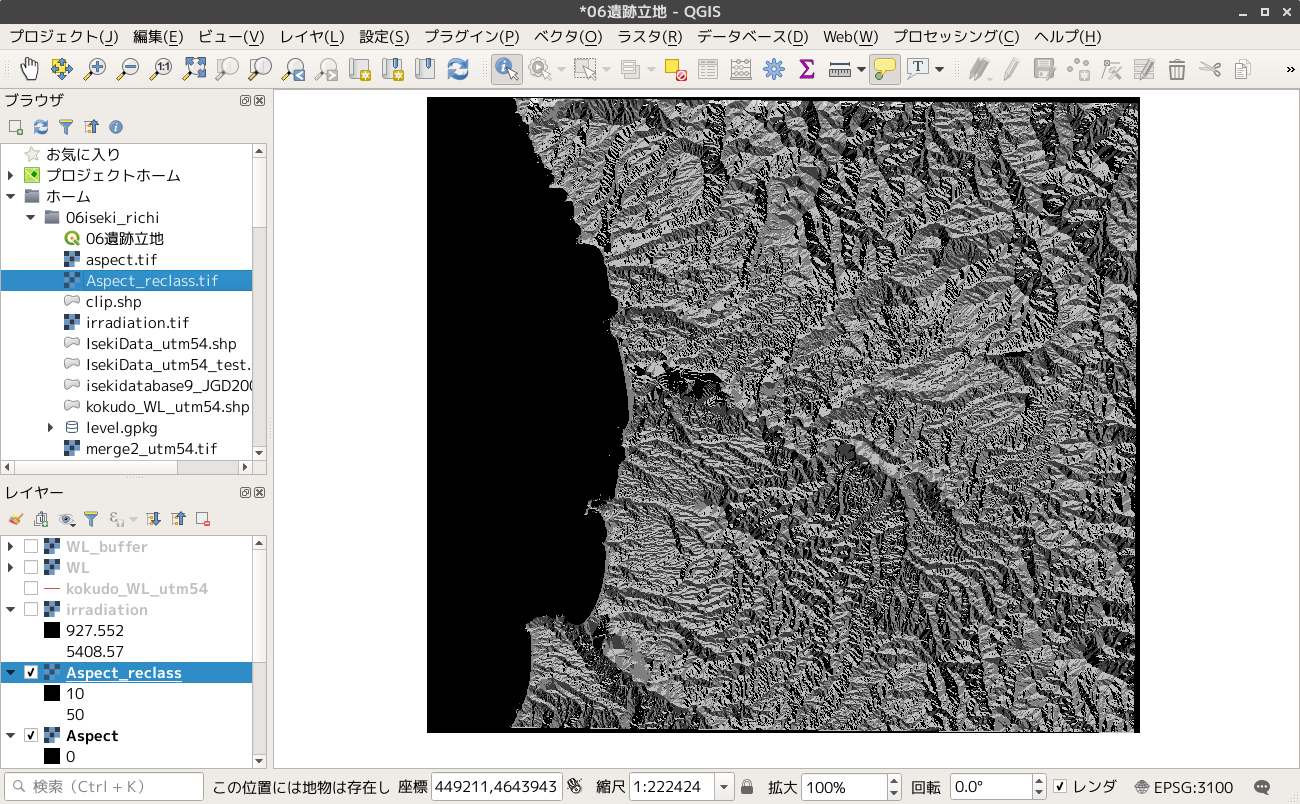
\includegraphics[width=1\linewidth]{38.png}
\caption{四方位に分類された傾斜方位ラスタ}
\end{figurehere}


%%%%
\section{ラスタのポリゴン化}
離散量化した方イラスタをベクタポリゴンに変換します。離散量の場合、データベースとして扱えるベクタデータに変換して利用するほうが有用なことが多いものです。なお、今回の分析方法ではラスタのままで作業するほうが処理速度が圧倒的に早くなります。

\begin{figurehere}
\centering
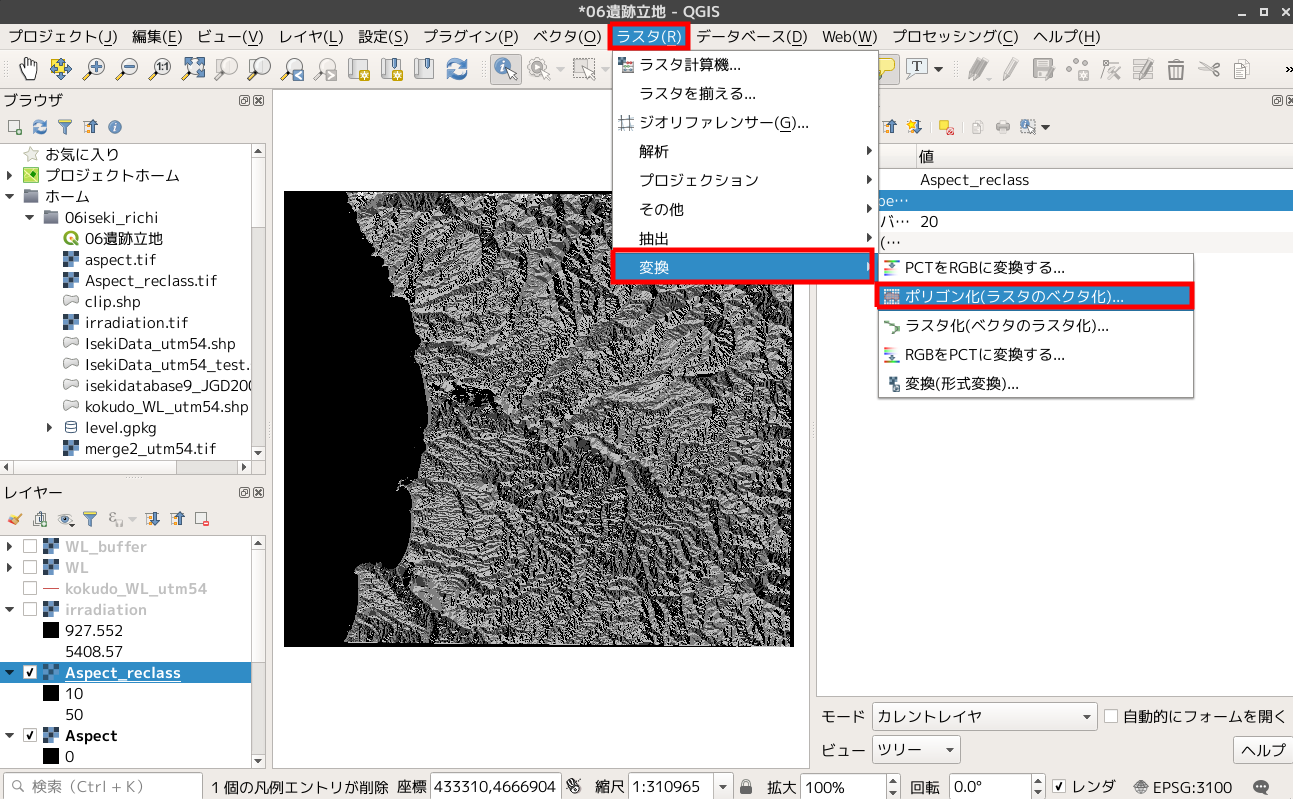
\includegraphics[width=1\linewidth]{39.png}
\caption{ラスタのベクタ化(ポリゴン化)}
\end{figurehere}

\begin{figurehere}
\centering
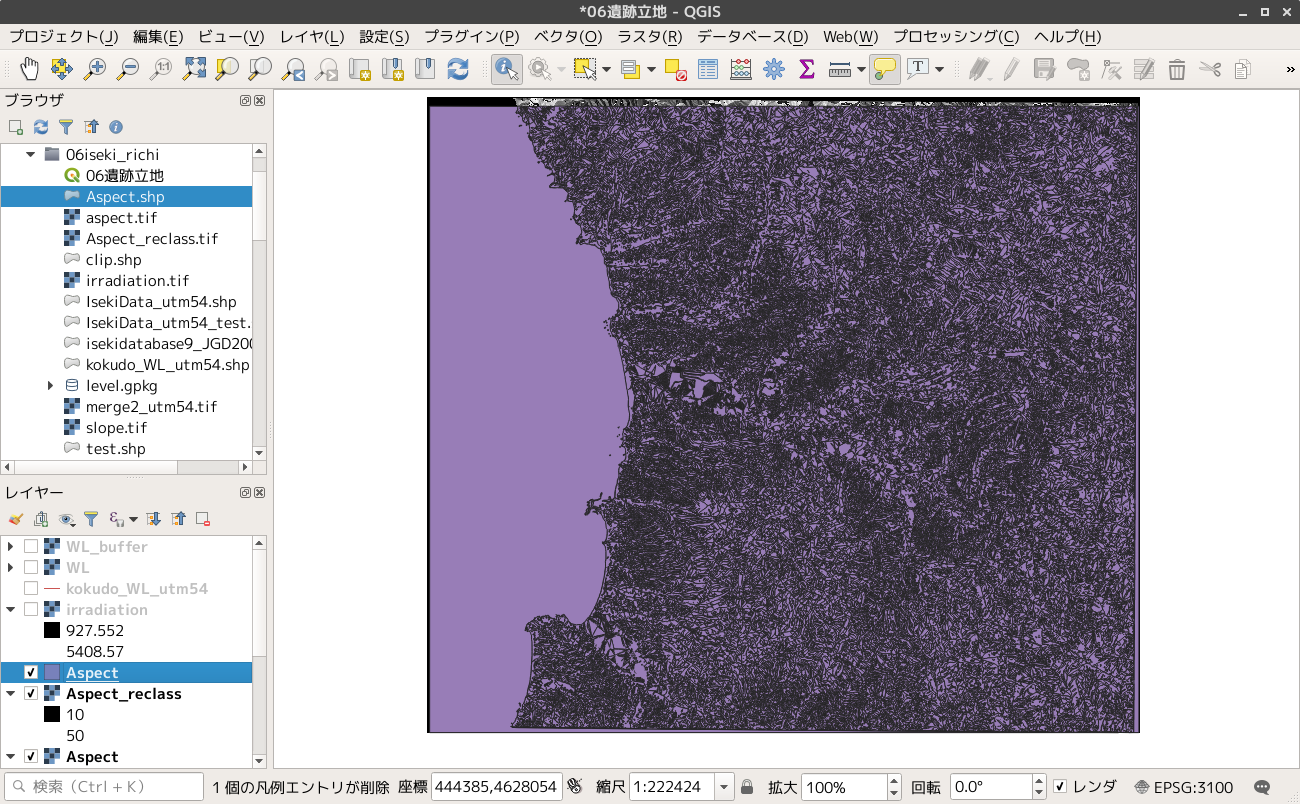
\includegraphics[width=1\linewidth]{40.png}
\caption{ポリゴン化された傾斜方位}
\end{figurehere}


%%%%
\section{フィールド計算機で方位を入れる}

作成した傾斜方位ベクタには方位を示す10とか20とかの数値が入っています。これを「東」「西」「南」「北」の文字列に置き換えます。こうした作業は「フィールド計算機」を使ったベクタ計算で行います。

\begin{enumerate}
\item 「出力フィールド名」→「aspect」
\item 「出力フィールドタイプ」→「string」
\end{enumerate}

\begin{figurehere}
\centering
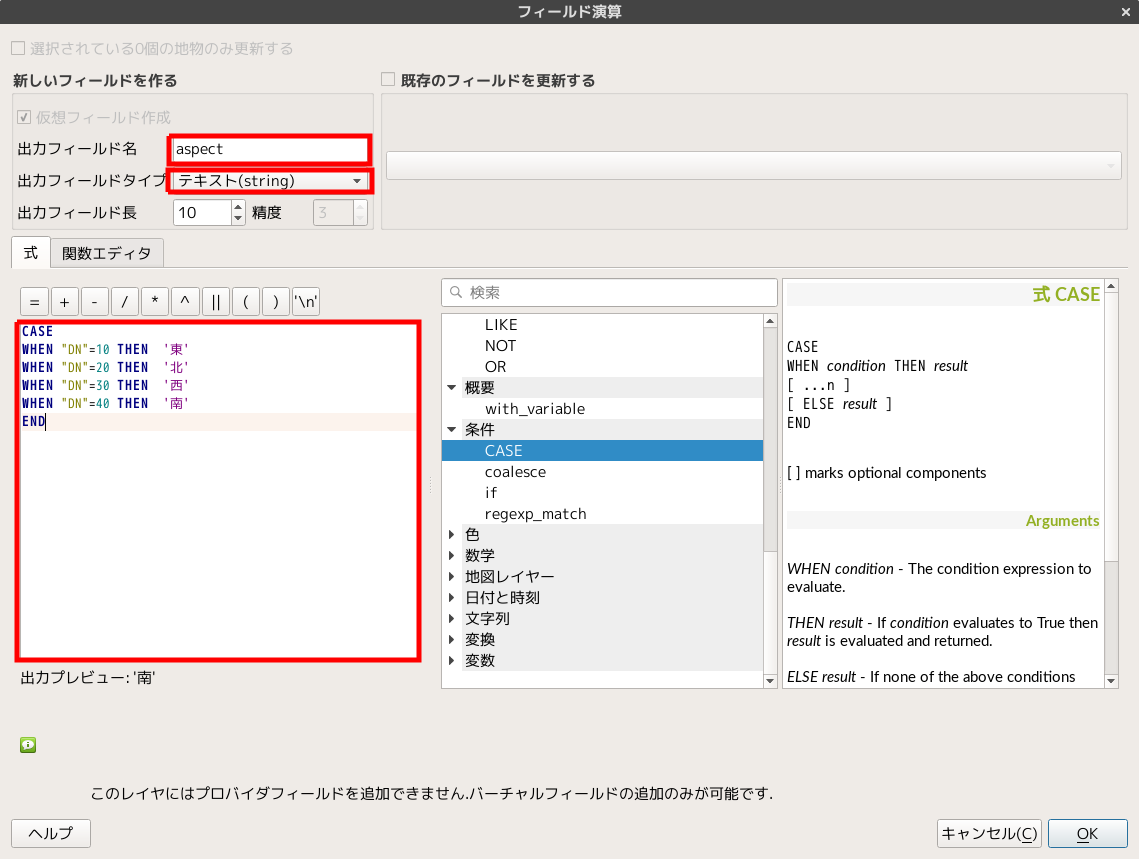
\includegraphics[width=0.8\linewidth]{42.png}
\caption{フィールド計算機}
\end{figurehere}

構文は次のとおりです。\\
$
CASE\\
WHEN 条件式 THEN 入力値\\
END
$

DNフィールド値が「10」なら「東」、「20」なら「北」・・・と指定していきます。\\
$
CASE\\
WHEN "DN"=10 THEN '東'\\
WHEN "DN"=20 THEN '北'\\
WHEN "DN"=30 THEN '西'\\
WHEN "DN"=40 THEN '南'\\
END
$
\vspace{1\baselineskip}

\begin{figurehere}
\centering
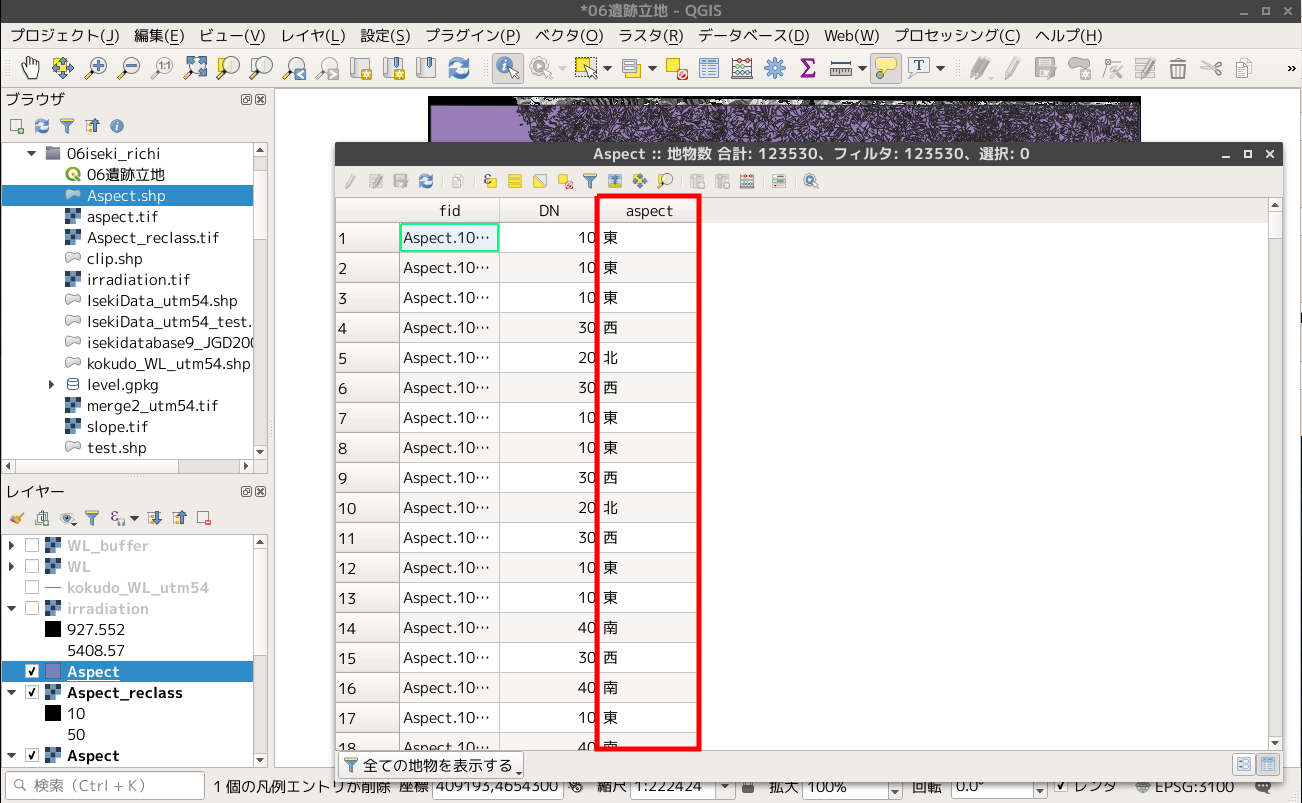
\includegraphics[width=0.8\linewidth]{43.png}
\caption{Aspectフィールドに文字列が代入される}
\end{figurehere}

%%%
\section{プラグインのインストール}
QGISには豊富な追加機能を提供するプラグインが用意されています。公式プラグインだけでも239件が登録されています。登録されたリポジトリからプラグインをえらんでダウンロードします。

\begin{enumerate}
\item 「プラグイン」→「プラグインの管理とインストール」
\item 「Point sampling tool」→「インストール」
\end{enumerate}

\begin{figurehere}
\centering
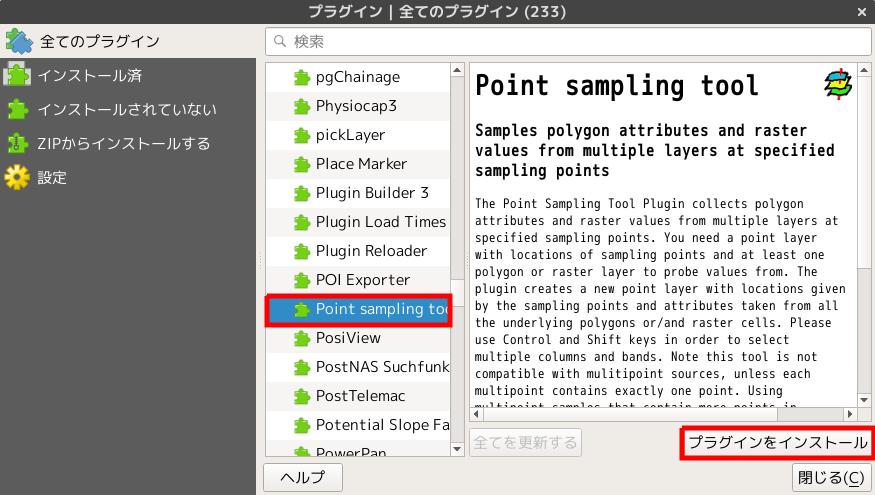
\includegraphics[width=0.8\linewidth]{04.png}
\caption{Point sampling toolをインストールする}
\end{figurehere}

%%%%
\section{Point sampling toolを使う}
「Point sampling tool」はポイントベクタレイヤと同じ座標の地形データを取得するためのプラグインです。ここでは遺跡立地地点の地形指標(標高や傾斜)を取得します。

\begin{enumerate}
\item 「プラグイン」→「Analysis」→「Point sampling tool」
\item 「General」タブを選択
\item サンプリングポイントレイヤに「IsekiData utm54」を選択
\item 値を取得したいレイヤを選択
\item 出力レイヤは「.gpkg」一択
\end{enumerate}

\begin{figurehere}
\centering
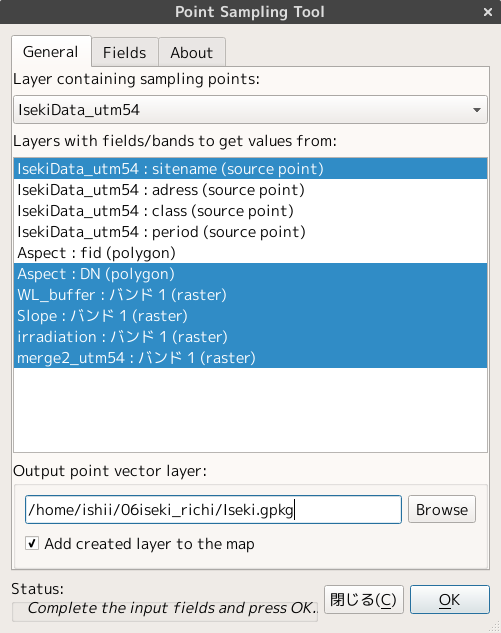
\includegraphics[width=0.7\linewidth]{06.png}
\caption{Point sampling toolの設定その1}
\end{figurehere}

\begin{enumerate}
\item 「Field」タブを選択
\item 「name」フィールドをわかりやすくリネーム
\end{enumerate}

\begin{figurehere}
\centering
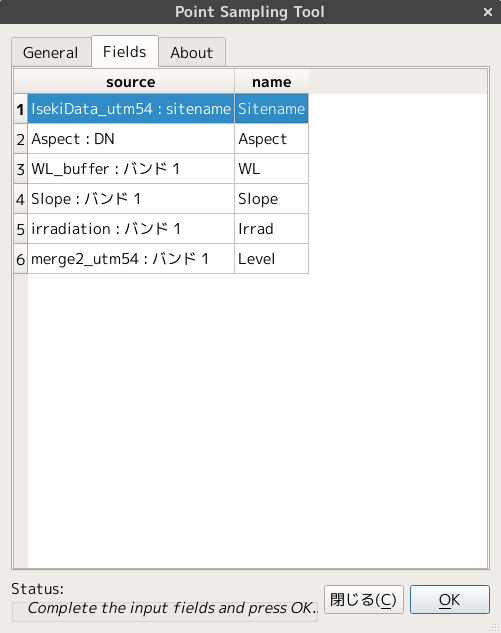
\includegraphics[width=0.7\linewidth]{07.png}
\caption{Point sampling toolの設定その2}
\end{figurehere}

\begin{figurehere}
\centering
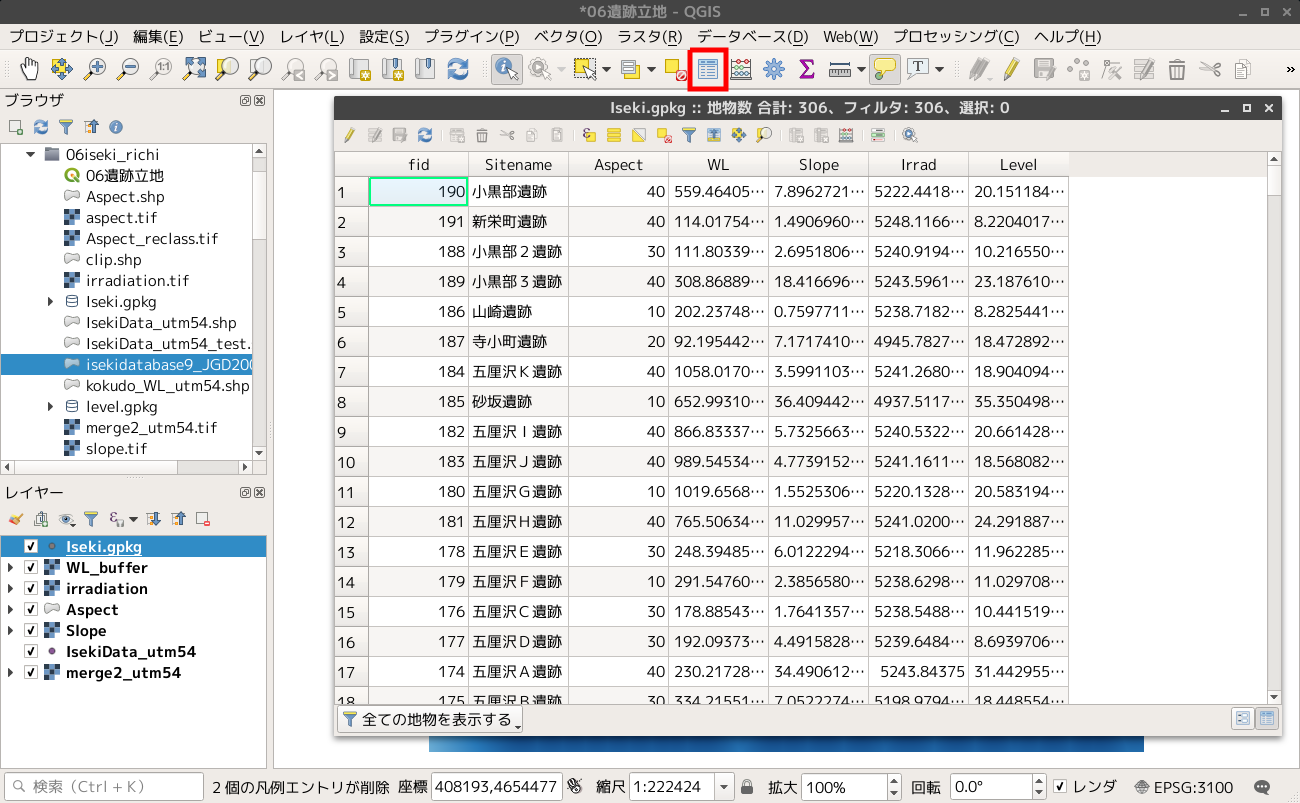
\includegraphics[width=0.7\linewidth]{45.png}
\caption{遺跡情報と地形情報が一つのデータに書き込まれた}
\end{figurehere}

%%%%
\section{GISデータを出力}
遺跡立地地点の地形データを表計算ソフトなどで扱えるcsv形式で出力します。csvに出力することでGIS以外のソフトウェアでGISデータを活用することができます。

\begin{itemize}
\item GISデータをcsvに出力する
\item 表計算ソフトで統計処理
\end{itemize}

\begin{enumerate}
\item 「Iseki.gpkg」→右クリック→「エクスポート」→「地物の保存」
\item 「形式」→「カンマで区切られた値[CSV]」
\item 「ファイル名」→「Iseki.csv」
\end{enumerate}

\begin{figurehere}
\centering
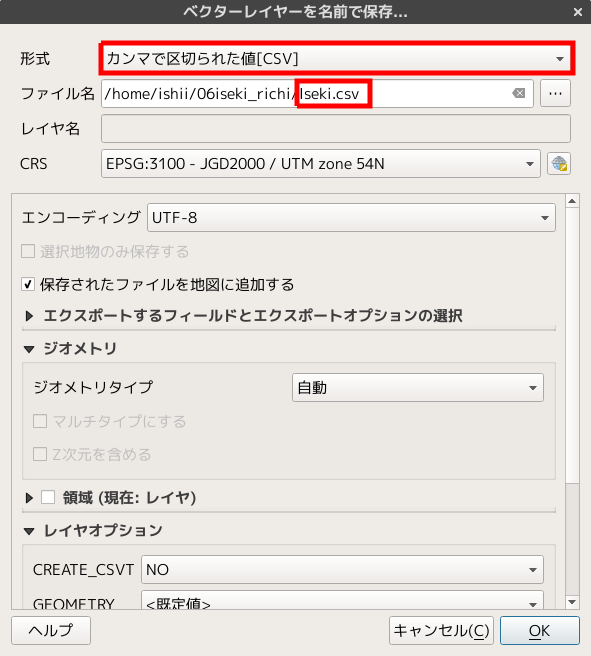
\includegraphics[width=0.7\linewidth]{48.png}
\caption{GISデータをcsvファイルに書き込む}
\end{figurehere}

\begin{figurehere}
\centering
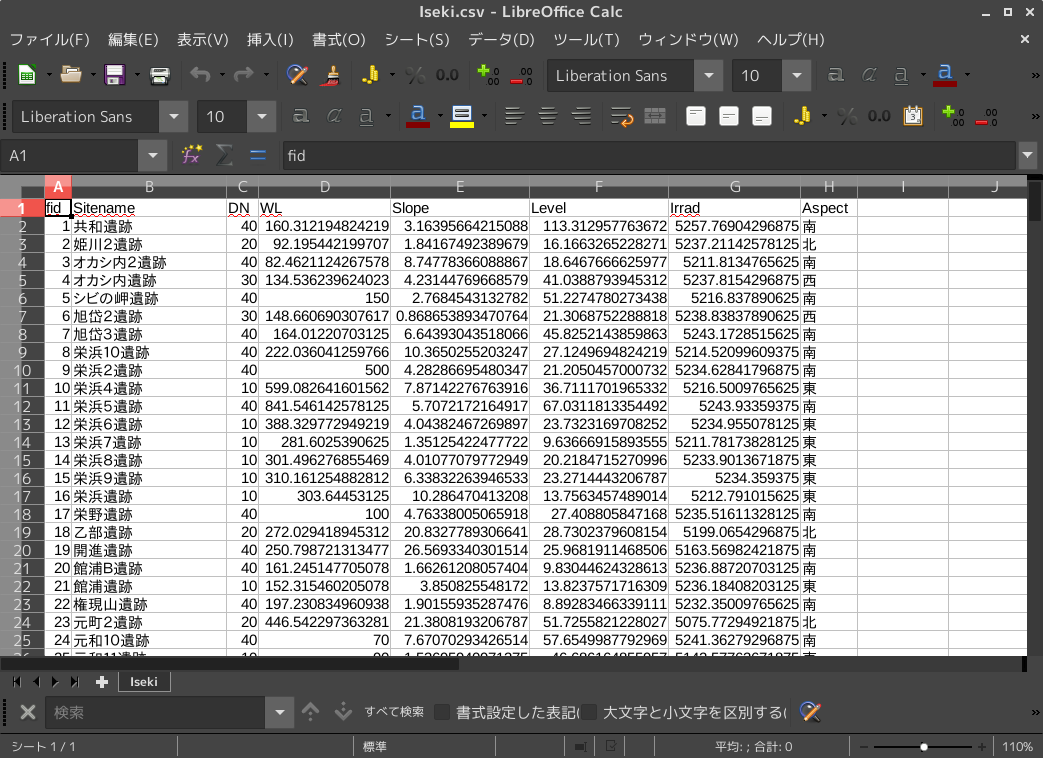
\includegraphics[width=\linewidth]{49.png}
\caption{表計算ソフトで開いたGISデータ}
\end{figurehere}

%%%%
\section{GIS統計データの可視化}
GISデータから遺跡立地の特徴を読み取るためには統計データの特徴を読み取ることが必要となります。表計算ソフトでは基本的な統計処理さえも複雑な手順を経る場合が多いので統計専用のソフトを利用することとなります。本研修では統計処理については触れませんので、あらかじめ作成したグラフを提示します。

また、可視化のためには変数の性質(連続量か離散量か)とその組み合わせを把握することが大切です。

\begin{itemize}
\item 連続量
	\begin{itemize}
	\item データの分布=ヒストグラム
	\item 2変量の関係=散布図
	\end{itemize}
\item 離散量
	\begin{itemize}
	\item 棒グラフ
	\end{itemize}
\item 連続量×離散量
	\begin{itemize}
	\item データの分布=ヒストグラム、箱ひげ図
	\end{itemize}
\item 離散量×離散量
	\begin{itemize}
	\item 積み上げ棒グラフ
	\end{itemize}
\end{itemize}

\begin{figurehere}
\centering
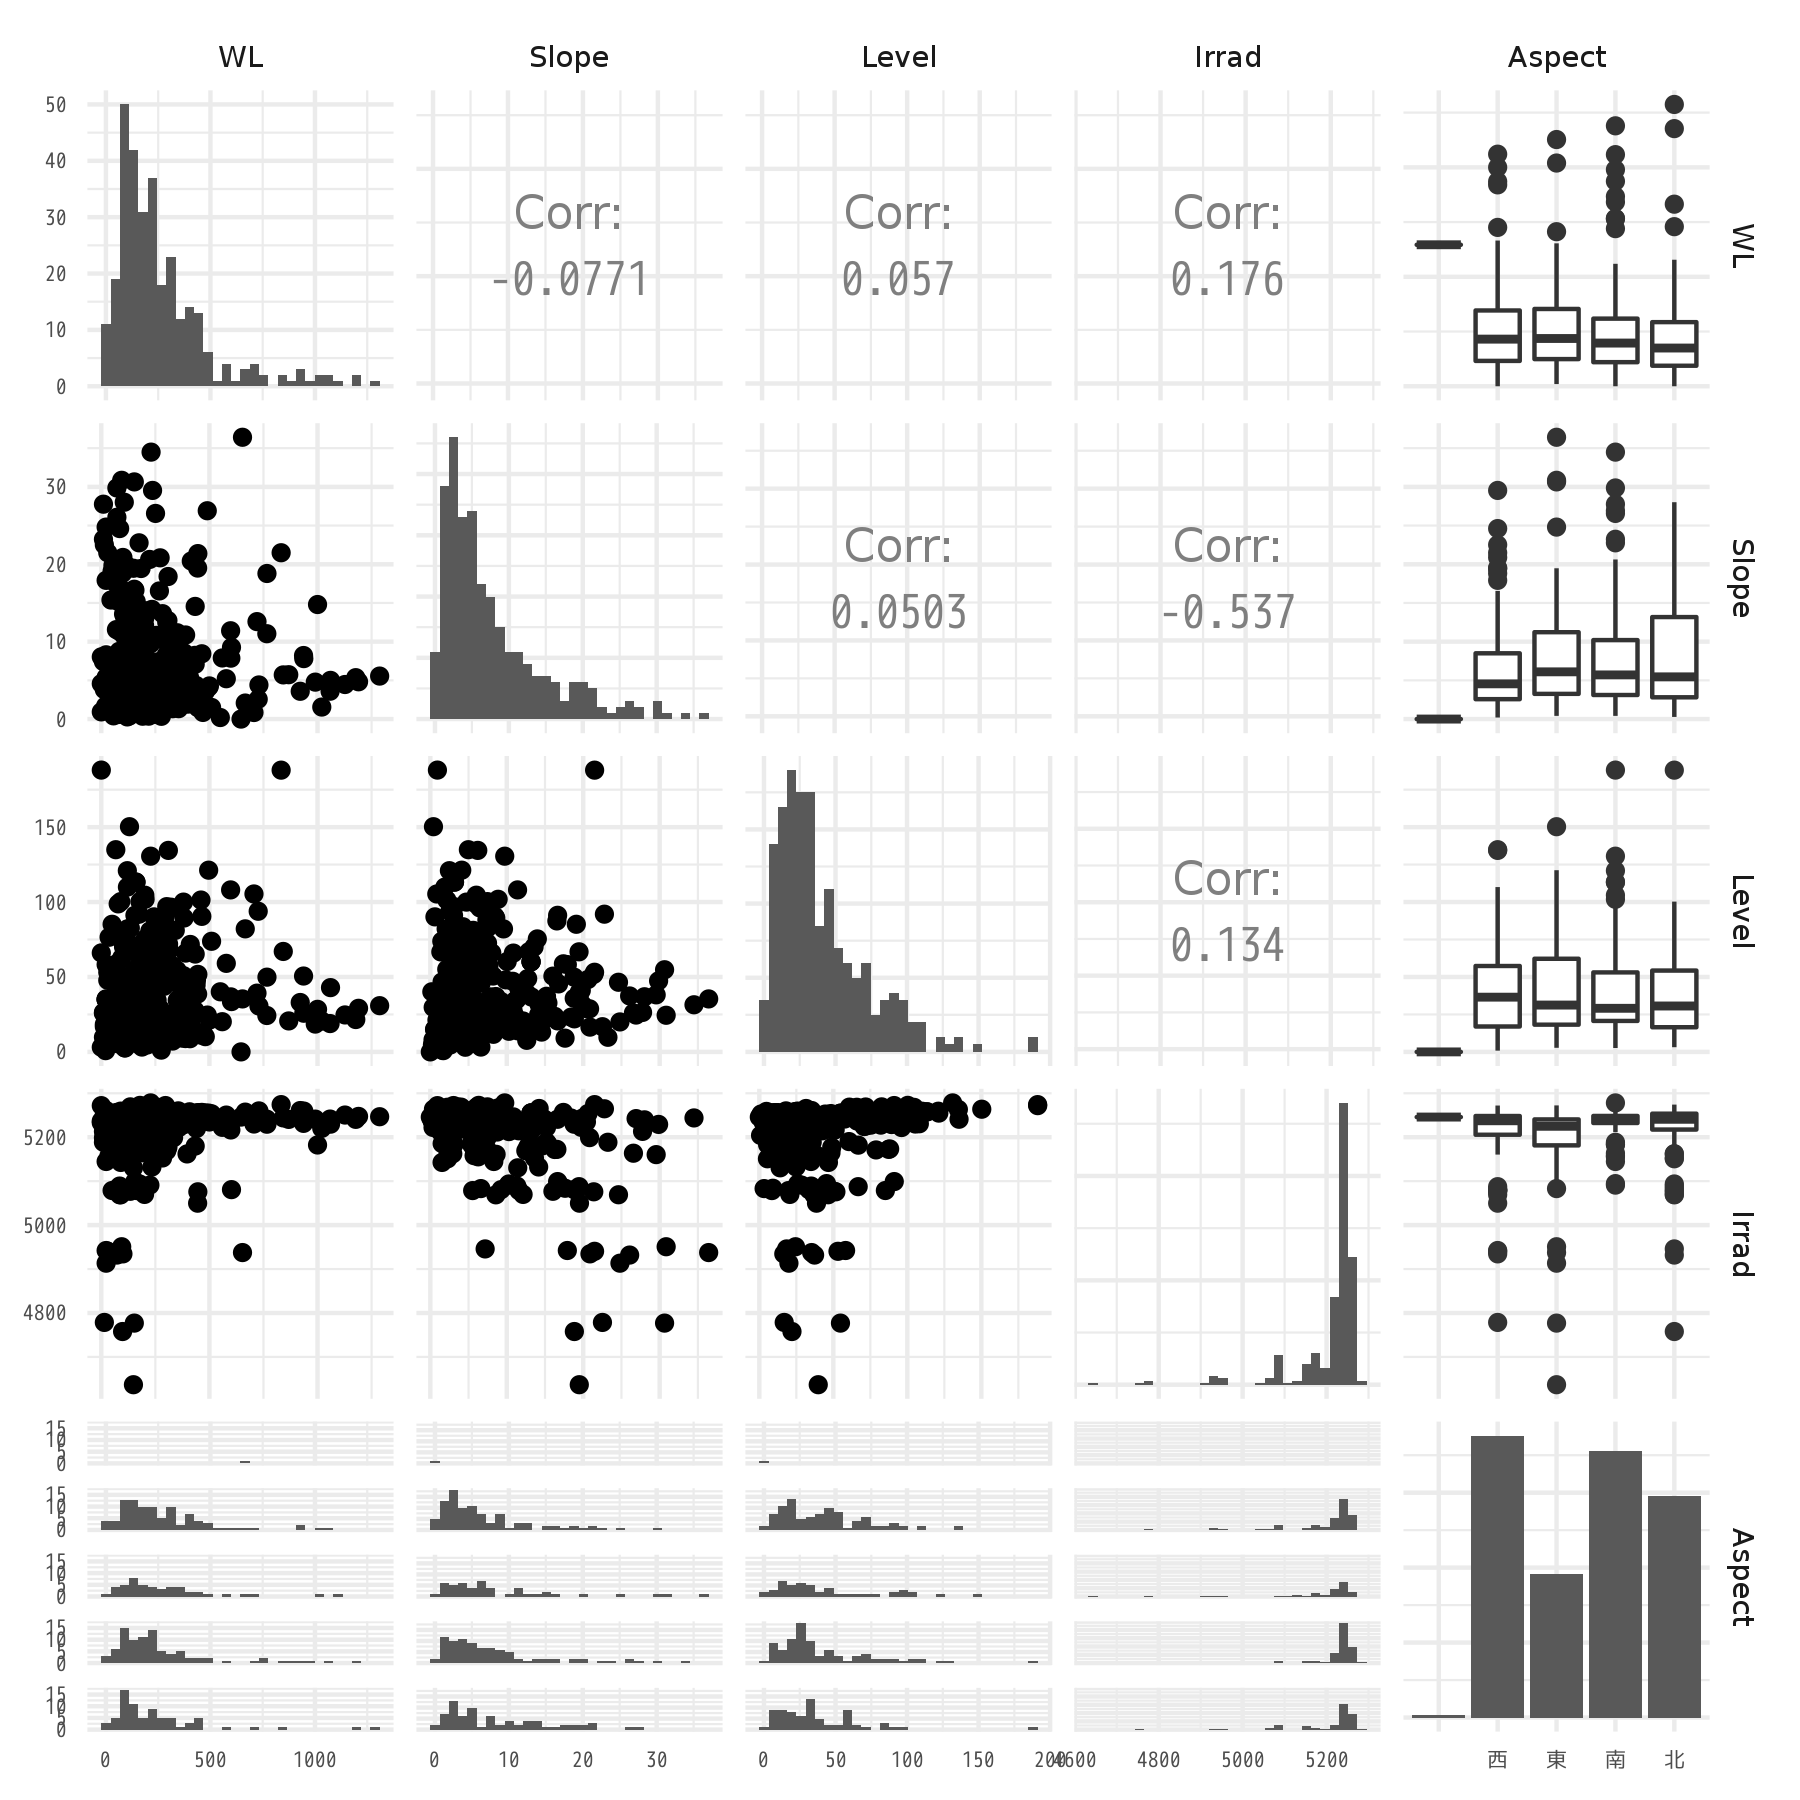
\includegraphics[width=0.8\linewidth]{R_graph/graph01.png}
\caption{地形データの要約}
\end{figurehere}

\begin{figurehere}
\centering
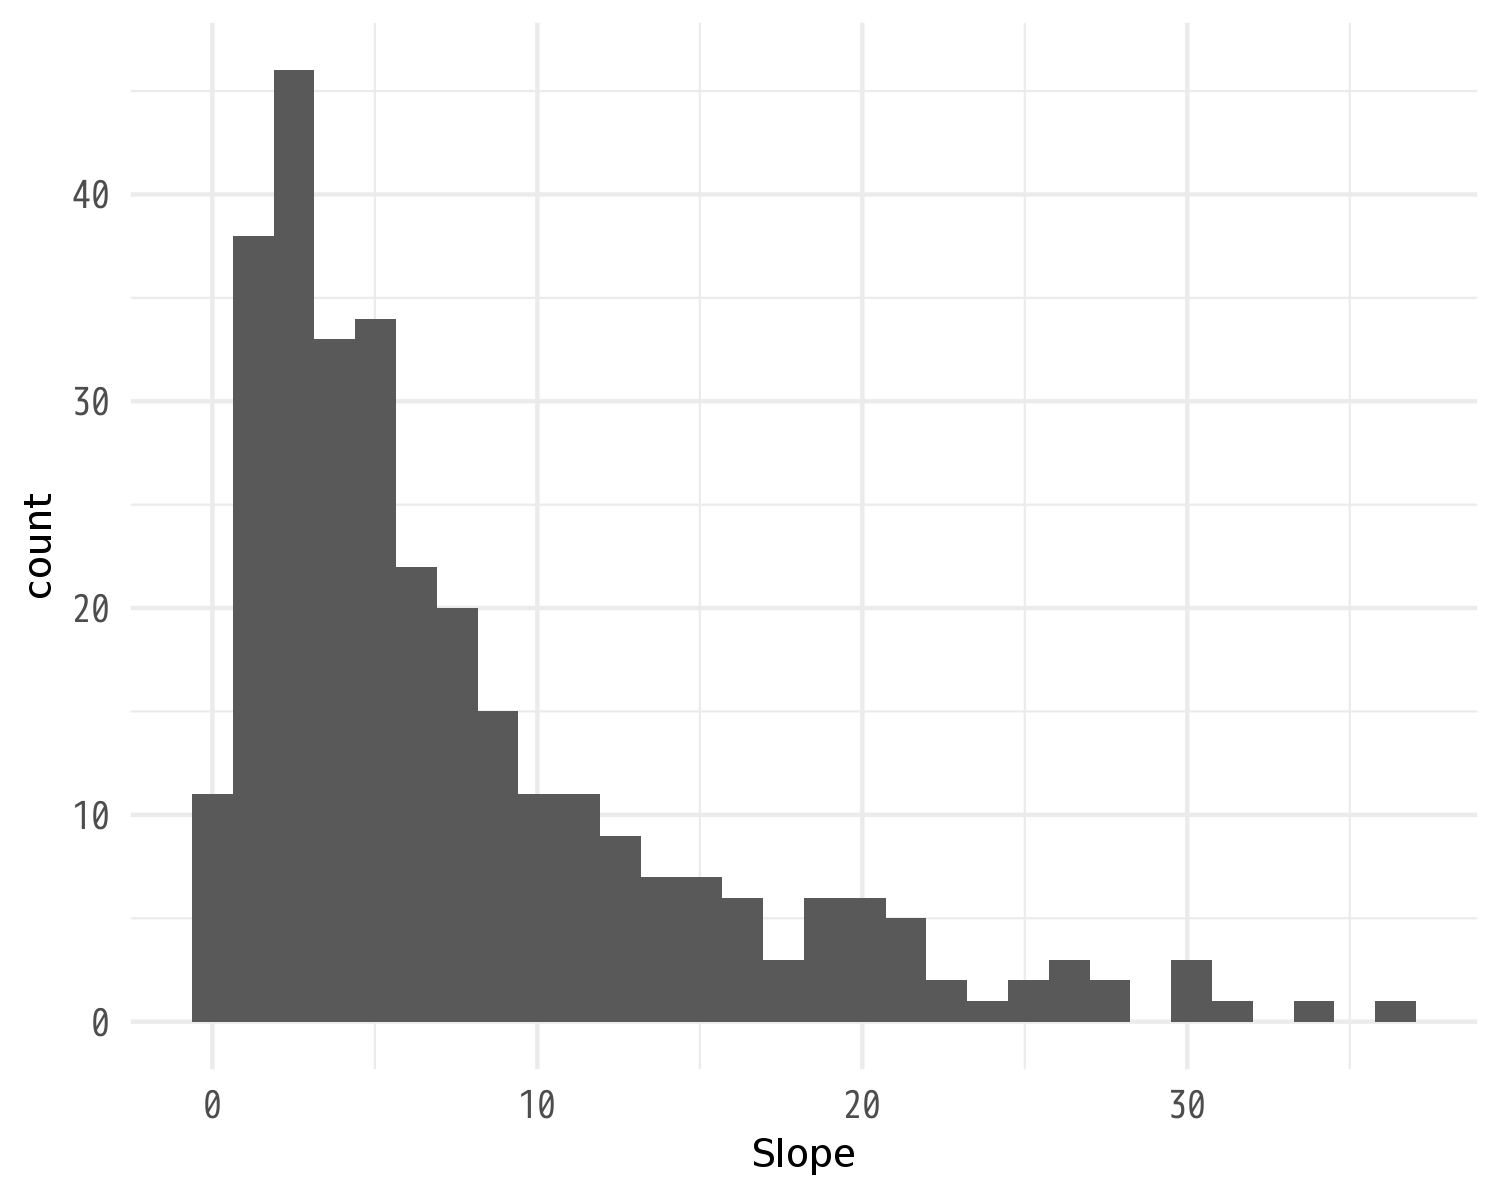
\includegraphics[width=0.8\linewidth]{R_graph/graph02.png}
\caption{ヒストグラム(傾斜角度)}
\end{figurehere}

\begin{figurehere}
\centering
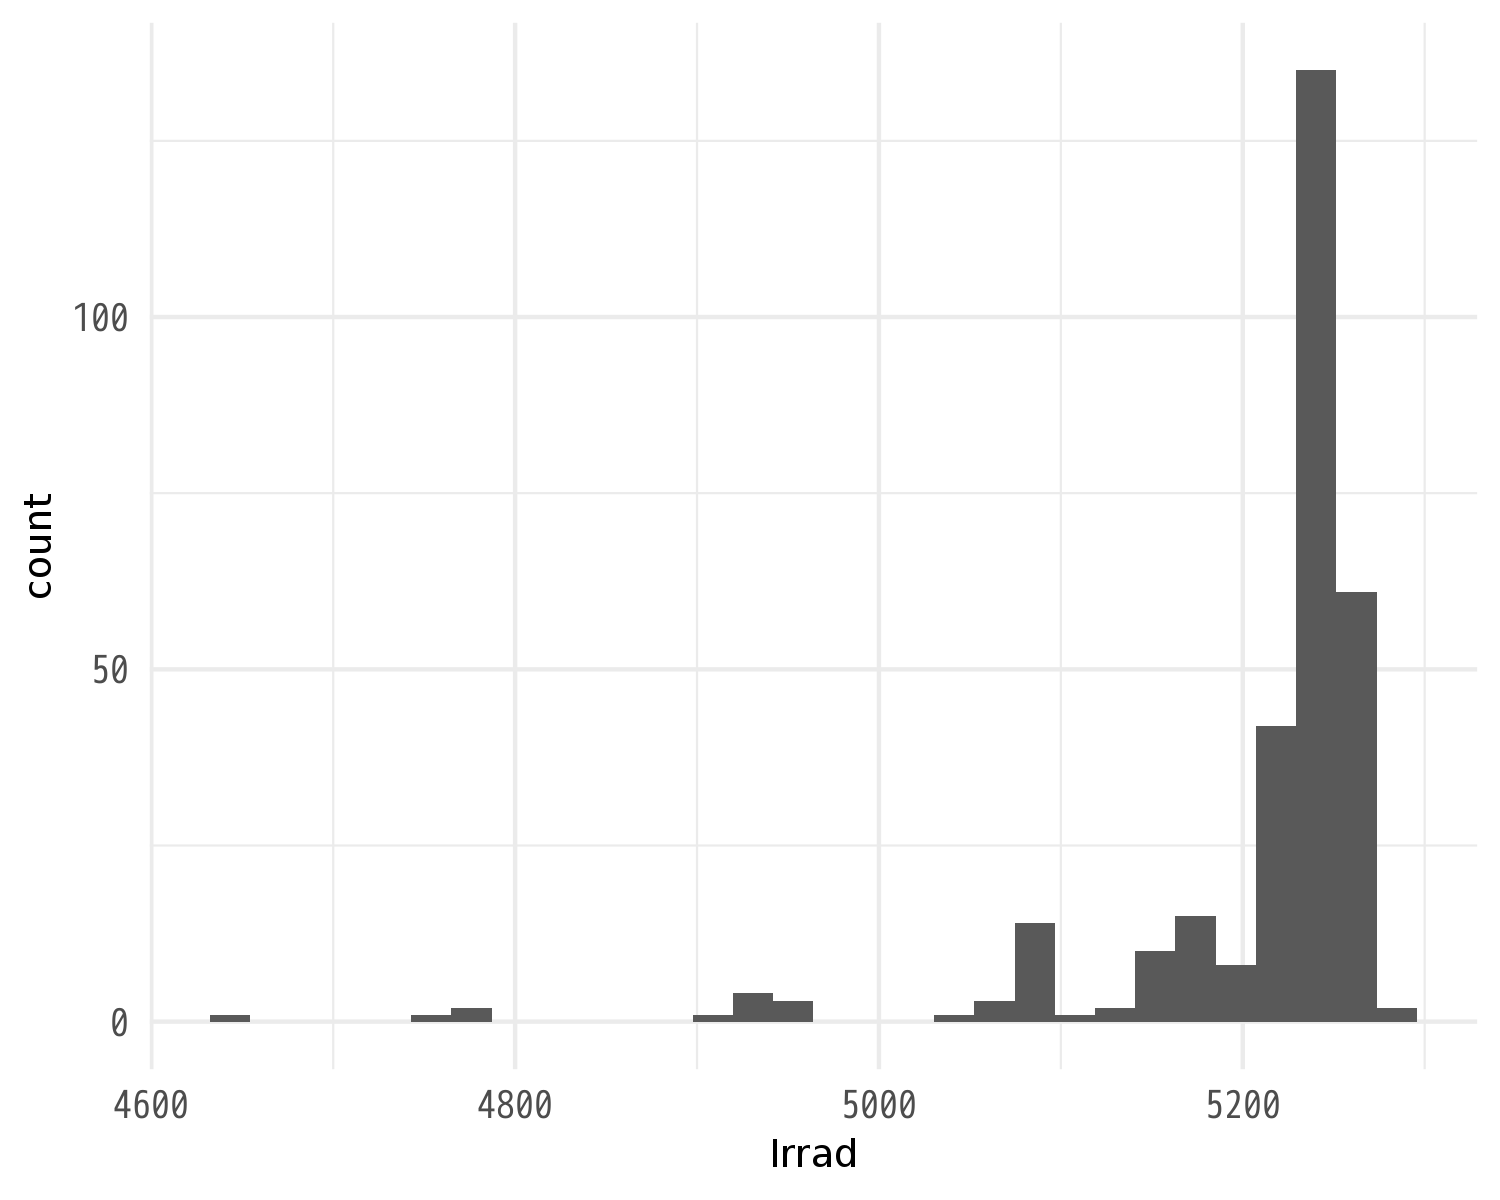
\includegraphics[width=0.8\linewidth]{R_graph/graph03.png}
\caption{ヒストグラム(日射量)}
\end{figurehere}

\begin{figurehere}
\centering
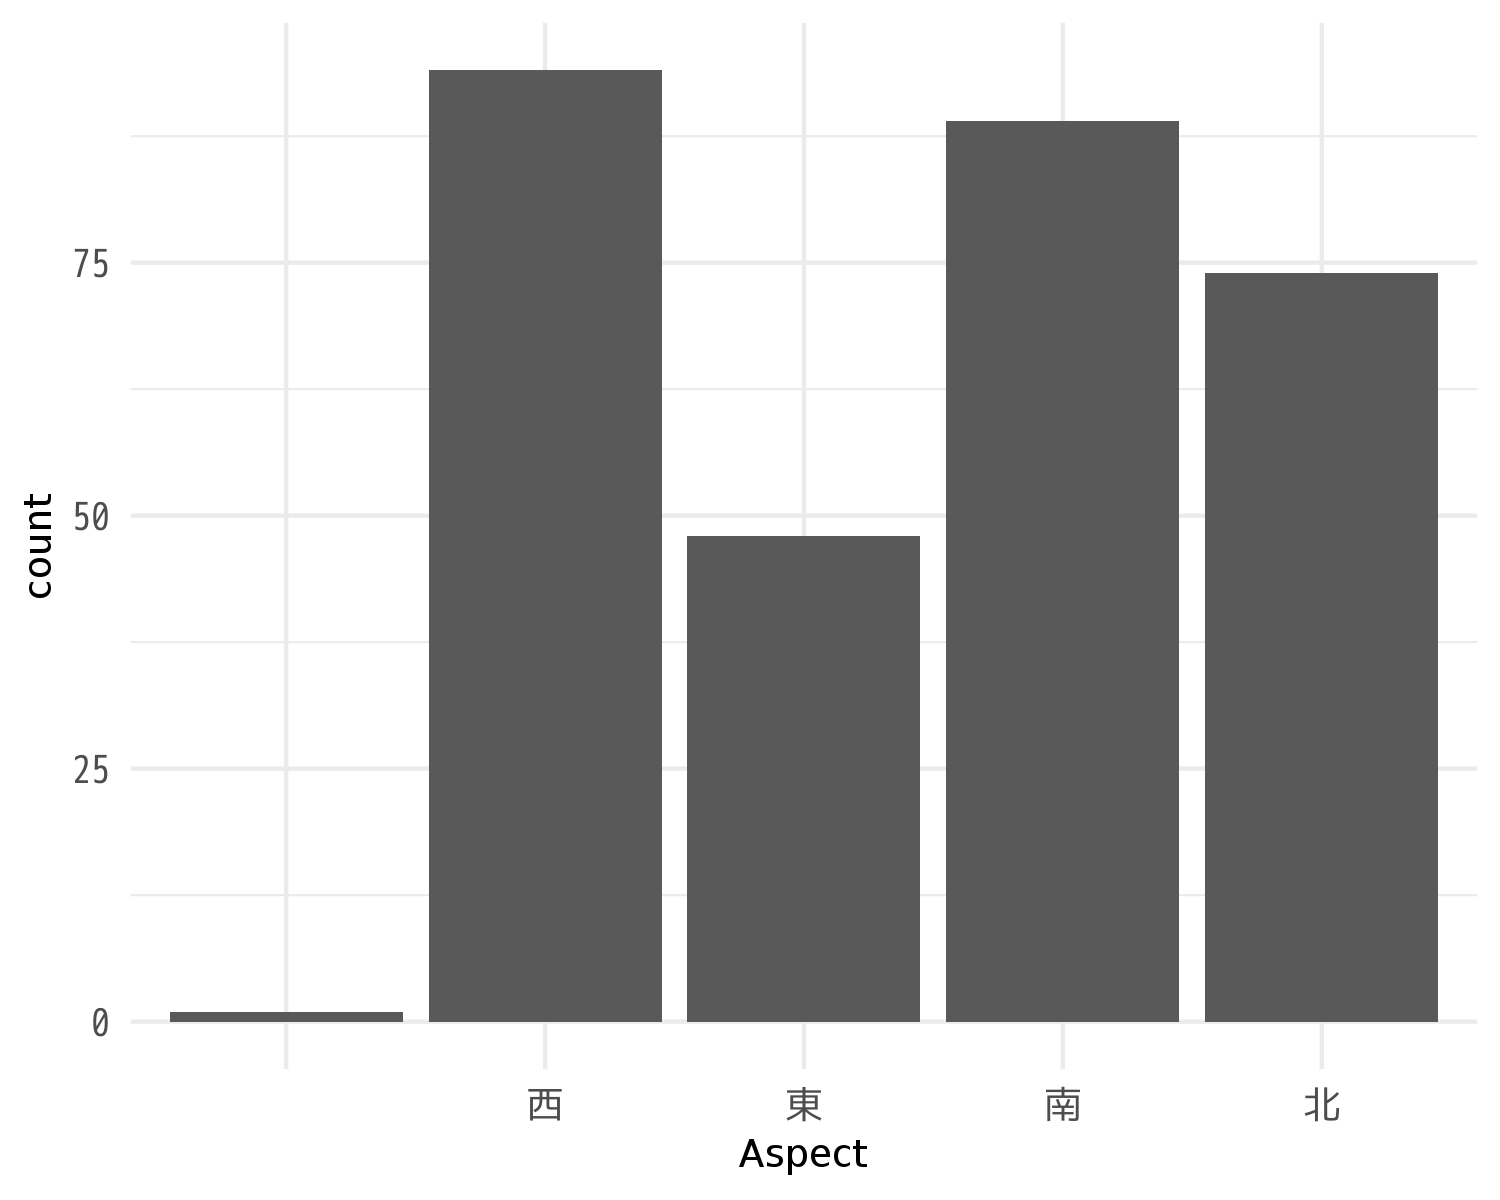
\includegraphics[width=0.8\linewidth]{R_graph/graph04.png}
\caption{棒グラフ(斜面方位)}
\end{figurehere}

%%%
\section{ランダムポイントを発生させる}
遺跡のない領域の地形データと比較するために、ランダムポイントを対象区域に発生させます。

\begin{itemize}
\item ランダムポイント発生
\item ランダムポイントに地形情報を付与
\item 遺跡のデータと結合
\end{itemize}


\begin{enumerate}
\item 「Clipcoast.shp」(マスク用のベクタレイヤ)開く
\item 「ベクタ」→「調査ツール」→「ポリゴン内のランダムポイント」
\end{enumerate}

\begin{enumerate}
\item 「入力レイヤ」→「ClipAria」
\item 「サンプリング手法」→「ポイント数」
\item 「式」→「300」(遺跡数と同数)
\item 「ランダム点群」→ファイル名を「Random.shp」
\end{enumerate}

\begin{figurehere}
\centering
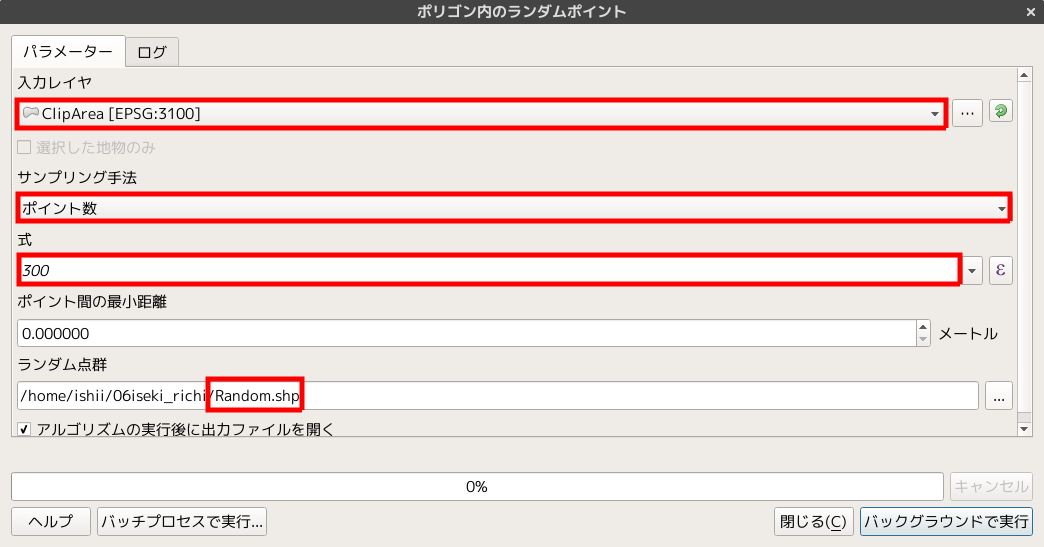
\includegraphics[width=1\linewidth]{52.png}
\caption{ポリゴン内のランダムポイントの設定}
\end{figurehere}

\begin{figurehere}
\centering
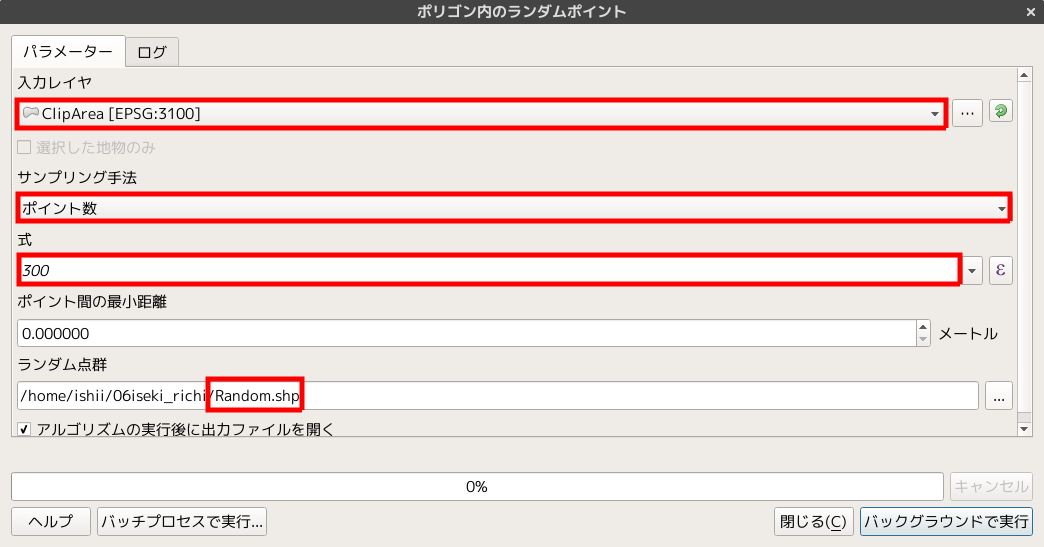
\includegraphics[width=1\linewidth]{52.png}
\caption{ポリゴンの領域にランダム点群を生成}
\end{figurehere}

%%%%
\section{再度「Point sampling tool」}
\begin{figurehere}
\centering
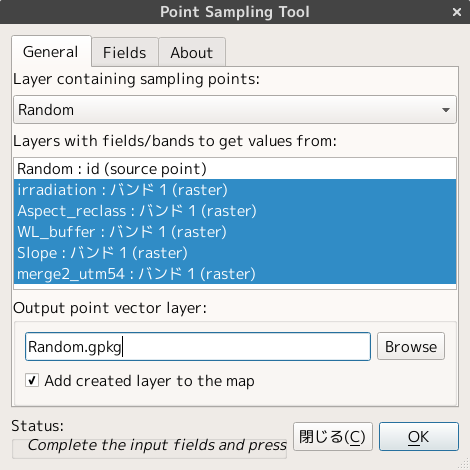
\includegraphics[width=1\linewidth]{54.png}
\caption{「Point sampling tool」の設定その1}
\end{figurehere}

\begin{figurehere}
\centering
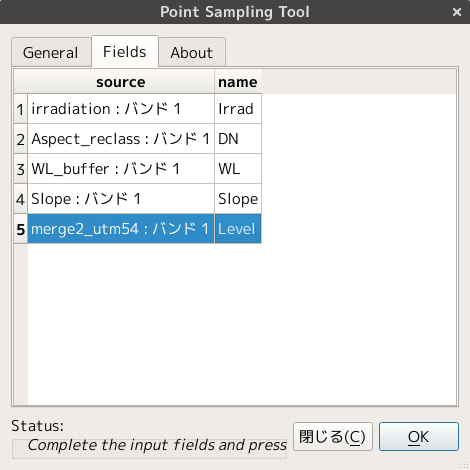
\includegraphics[width=1\linewidth]{55.png}
\caption{「Point sampling tool」の設定その2}
\end{figurehere}

%%%%
\section{csvに出力}
\begin{enumerate}
\item 地物を右クリック
\item 「形式」→「カンマで区切られた値[CSV]」
\item 「ファイル名」→「Random.csv」
\end{enumerate}

\begin{figurehere}
\centering
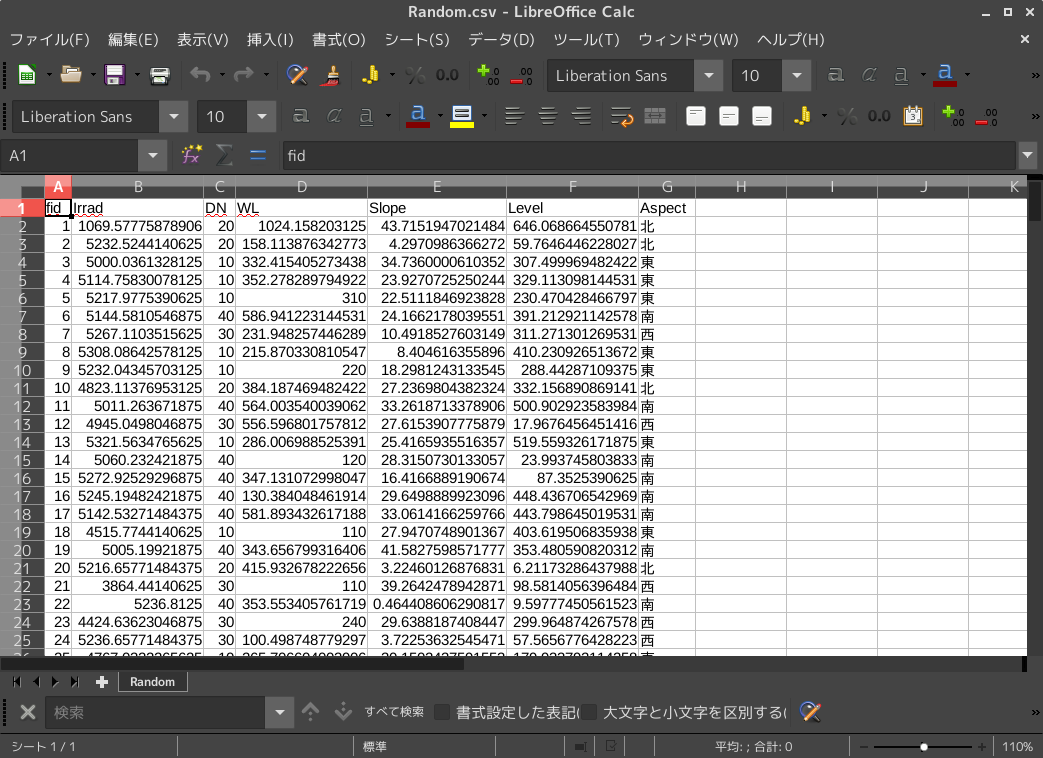
\includegraphics[width=1\linewidth]{58.png}
\caption{ランダム点群をcsvに出力}
\end{figurehere}

\begin{enumerate}
\item 先に作成した「Iseki.csv」と結合
\item 新たに「Class」カラムを作成して「遺跡」と「自然地形」を入力
\item 「Merge.csv」という名称で保存
\end{enumerate}

\begin{figurehere}
\centering
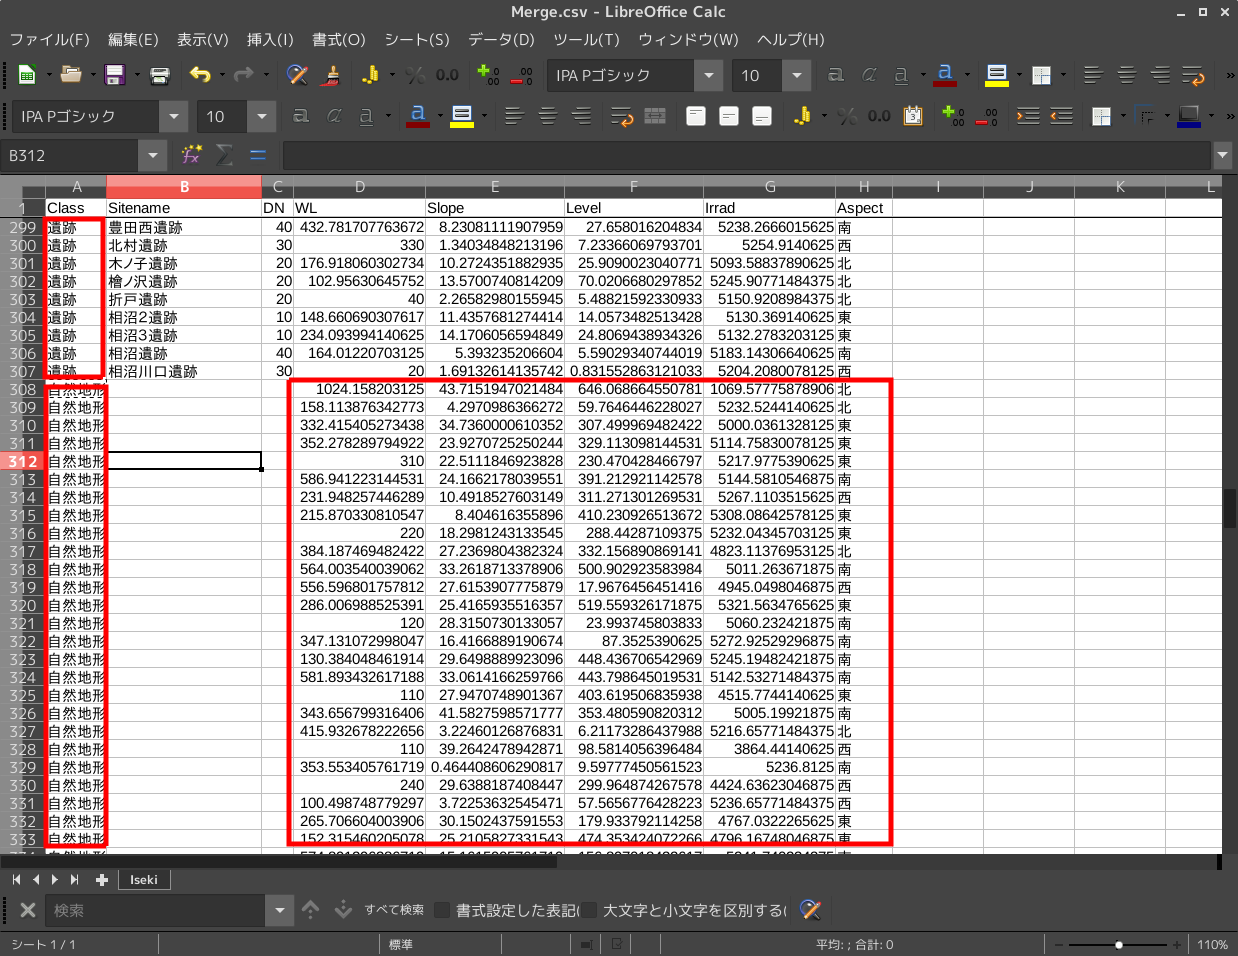
\includegraphics[width=1\linewidth]{59.png}
\caption{遺跡立地地点とランダム点群を結合}
\end{figurehere}

%%%%
\section{再び統計処理へ}
次のことについて調べたい。

\begin{itemize}
\item 遺跡立地に影響を与える地形指標を知りたい
\item 「遺跡の有無」という離散量に対して、それ以外の連続量や離散量がどのように影響するか。
\end{itemize}

\begin{figurehere}
\centering
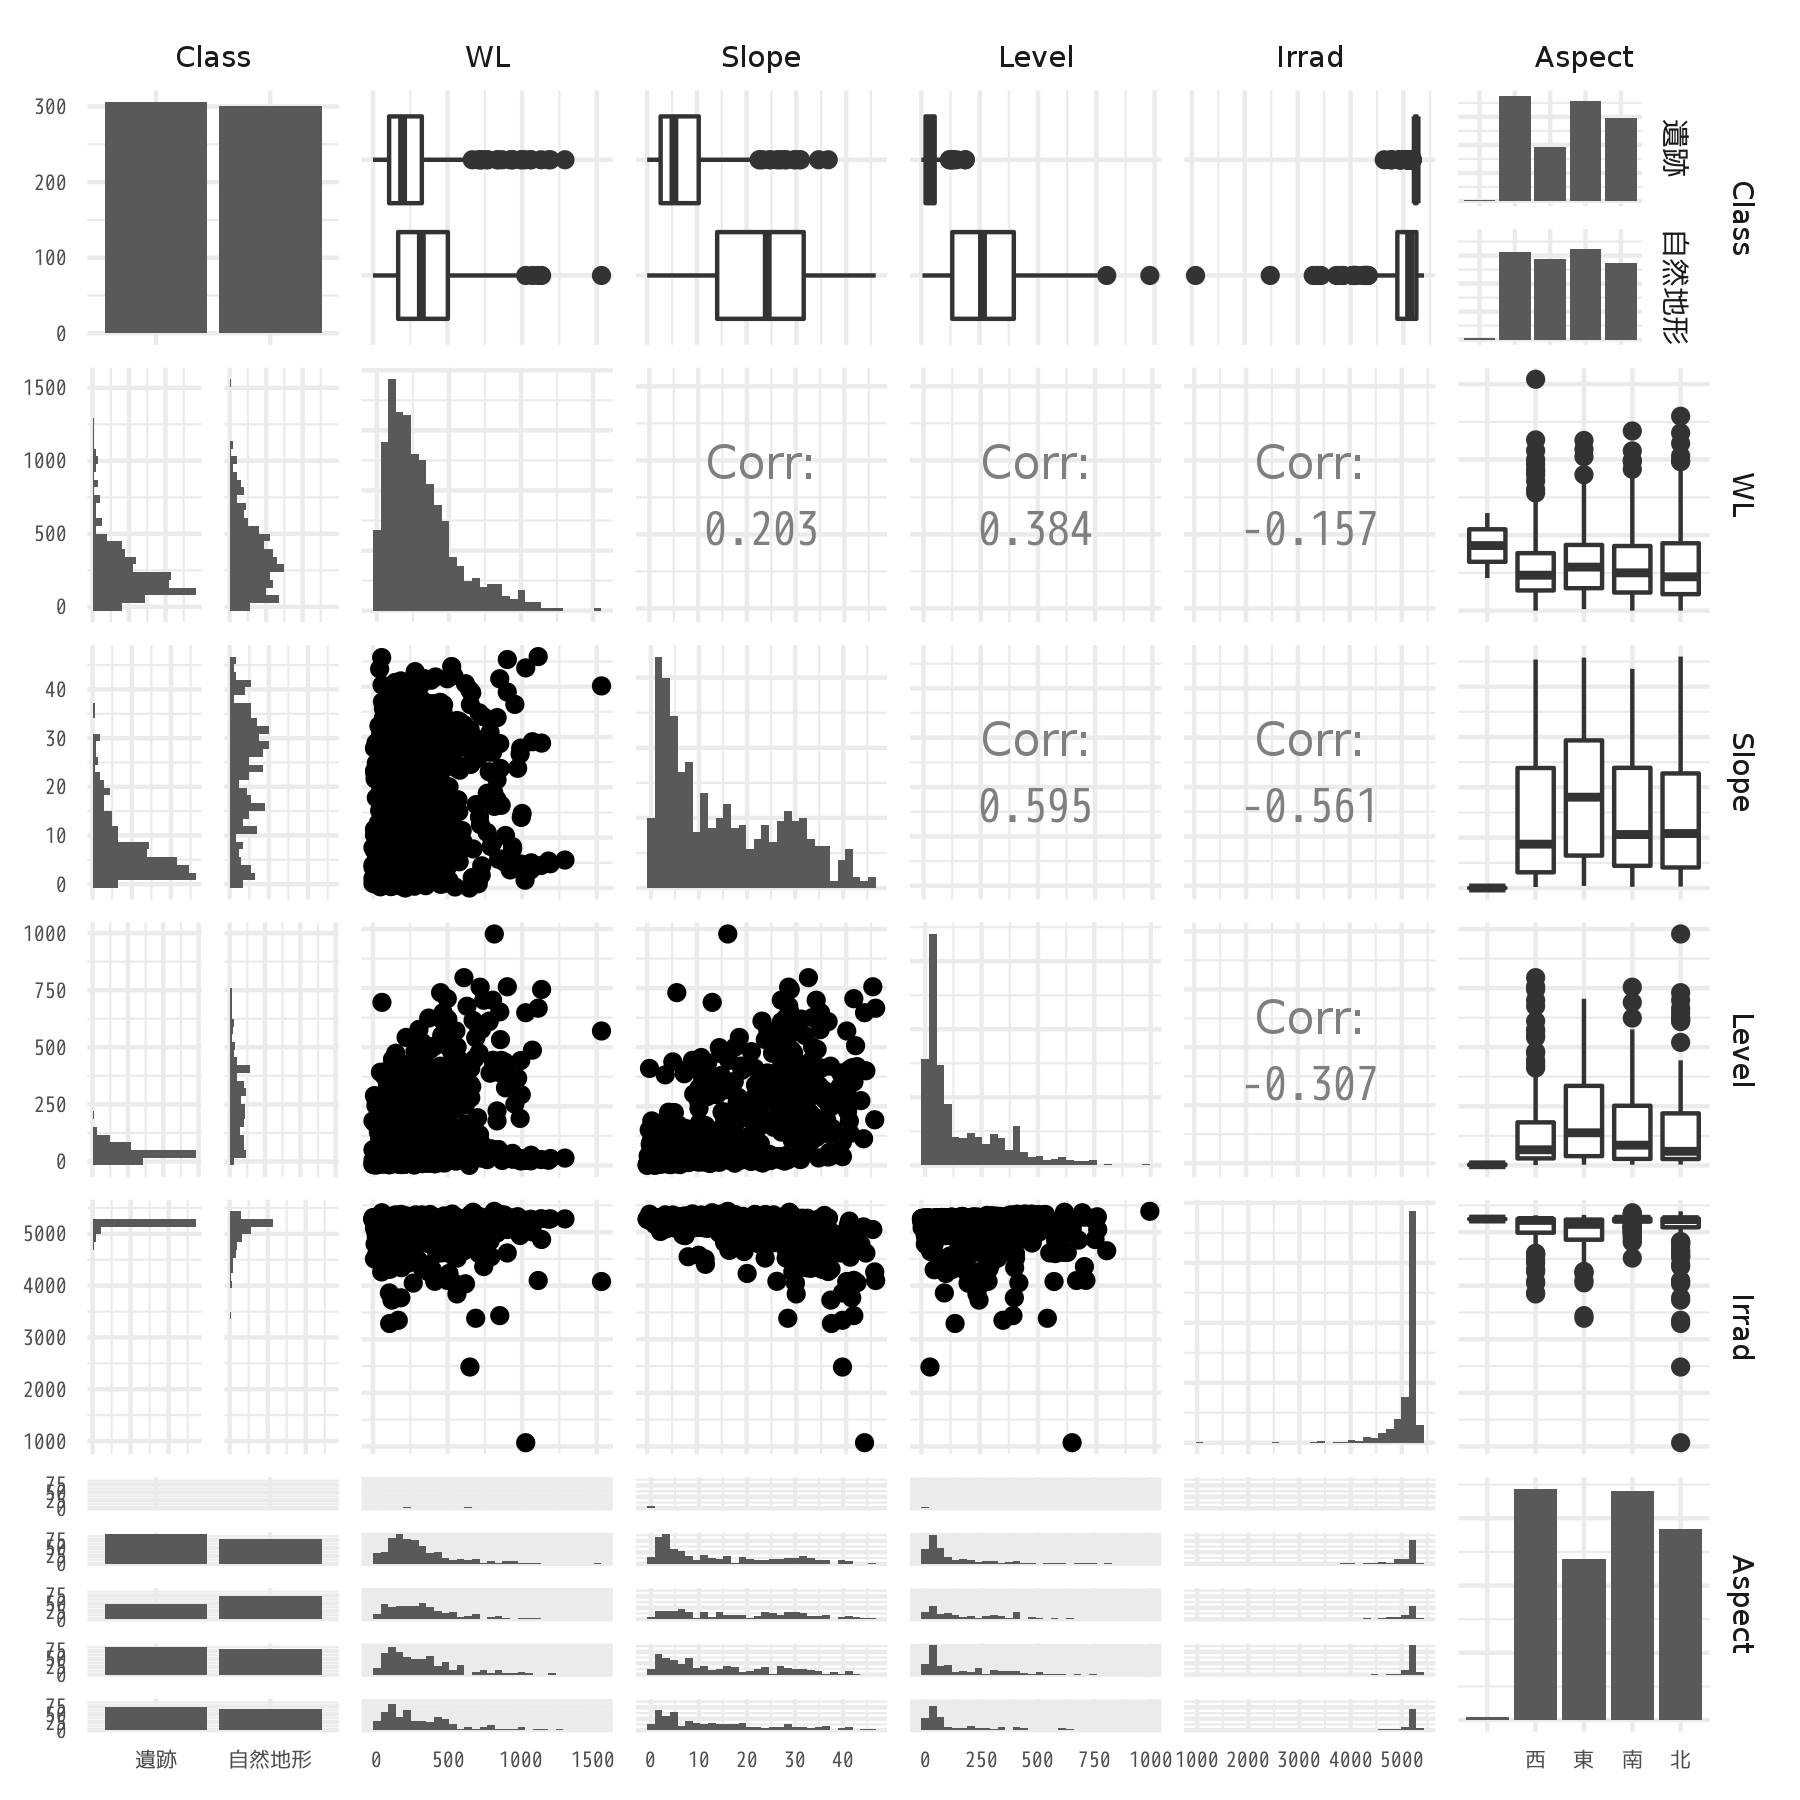
\includegraphics[width=0.8\linewidth]{R_graph/graph10.png}
\caption{データの概要を確認する}
\end{figurehere}

\begin{figurehere}
\centering
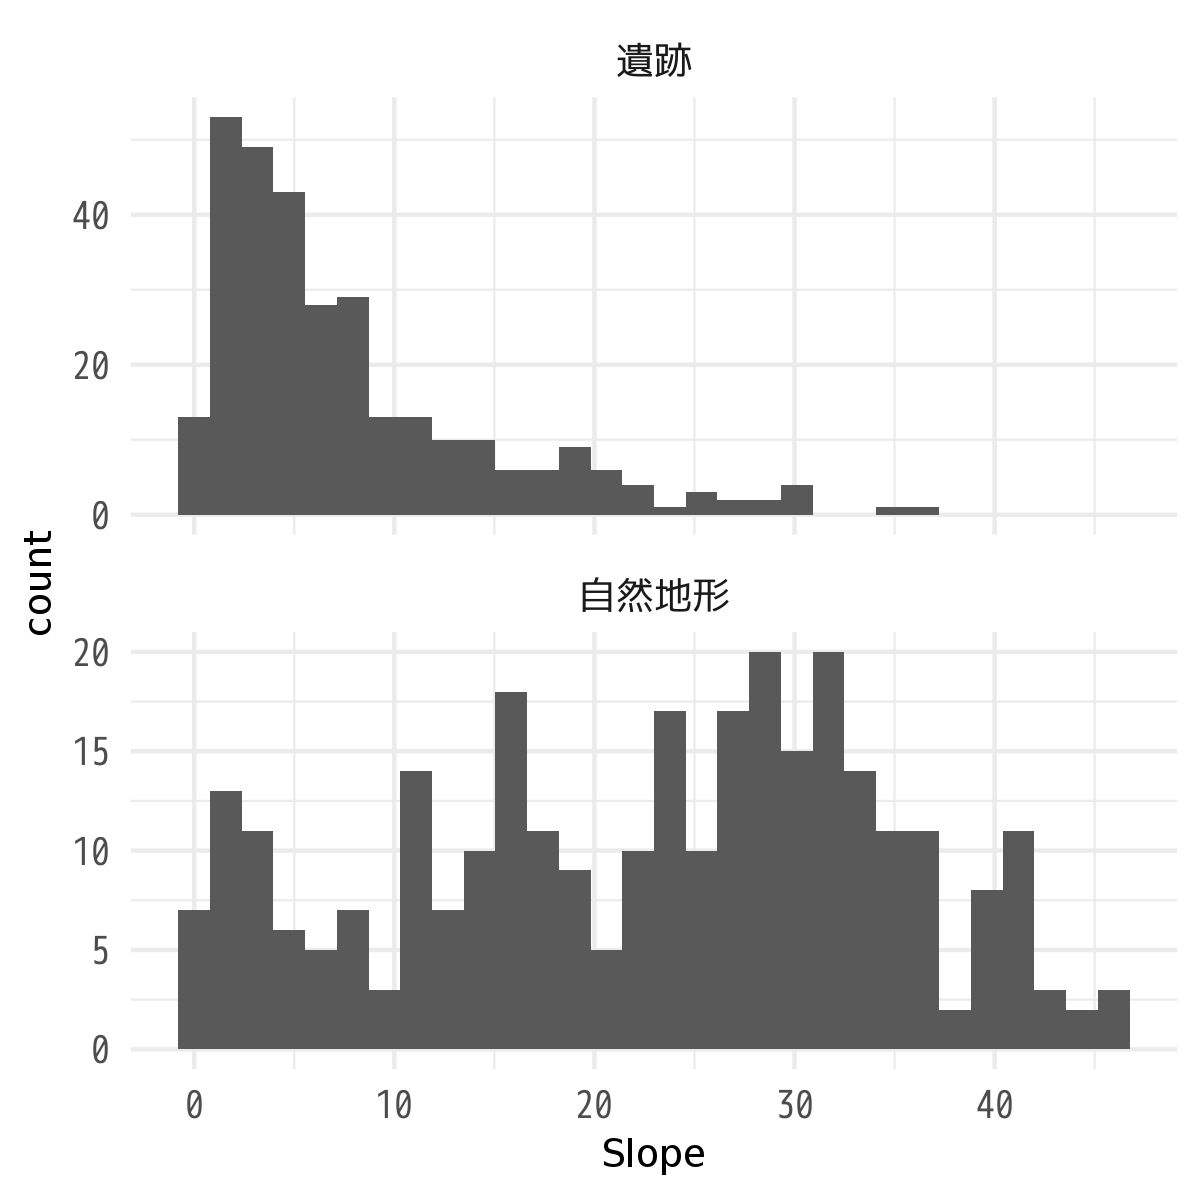
\includegraphics[width=1\linewidth]{R_graph/graph05.png}
\caption{傾斜}
\end{figurehere}

\begin{figurehere}
\centering
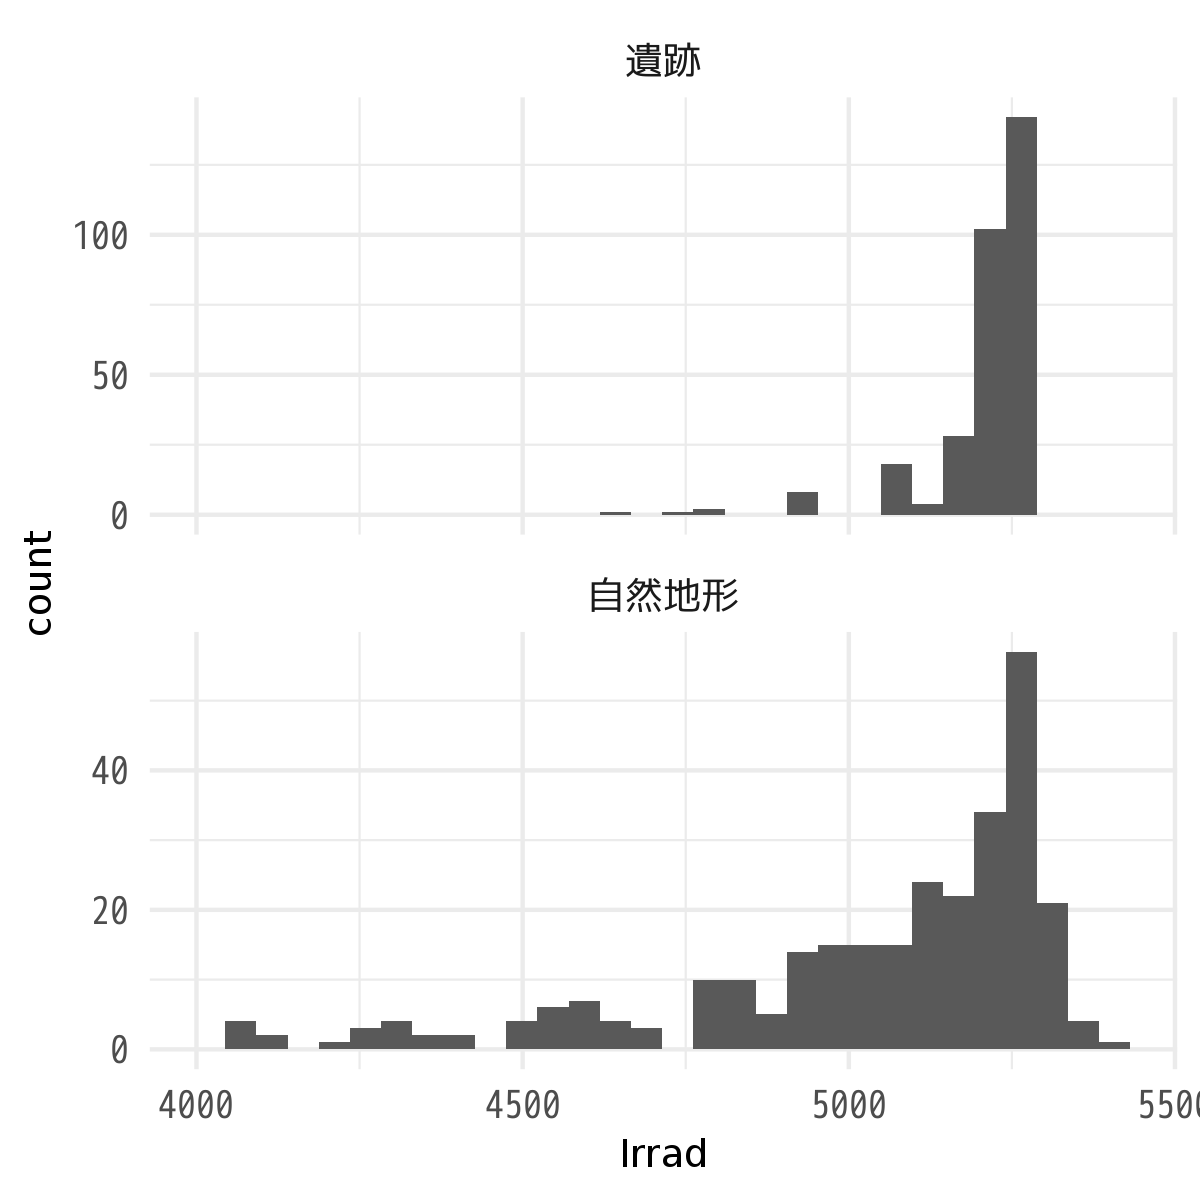
\includegraphics[width=1\linewidth]{R_graph/graph06.png}
\caption{日射量}
\end{figurehere}

\begin{figurehere}
\centering
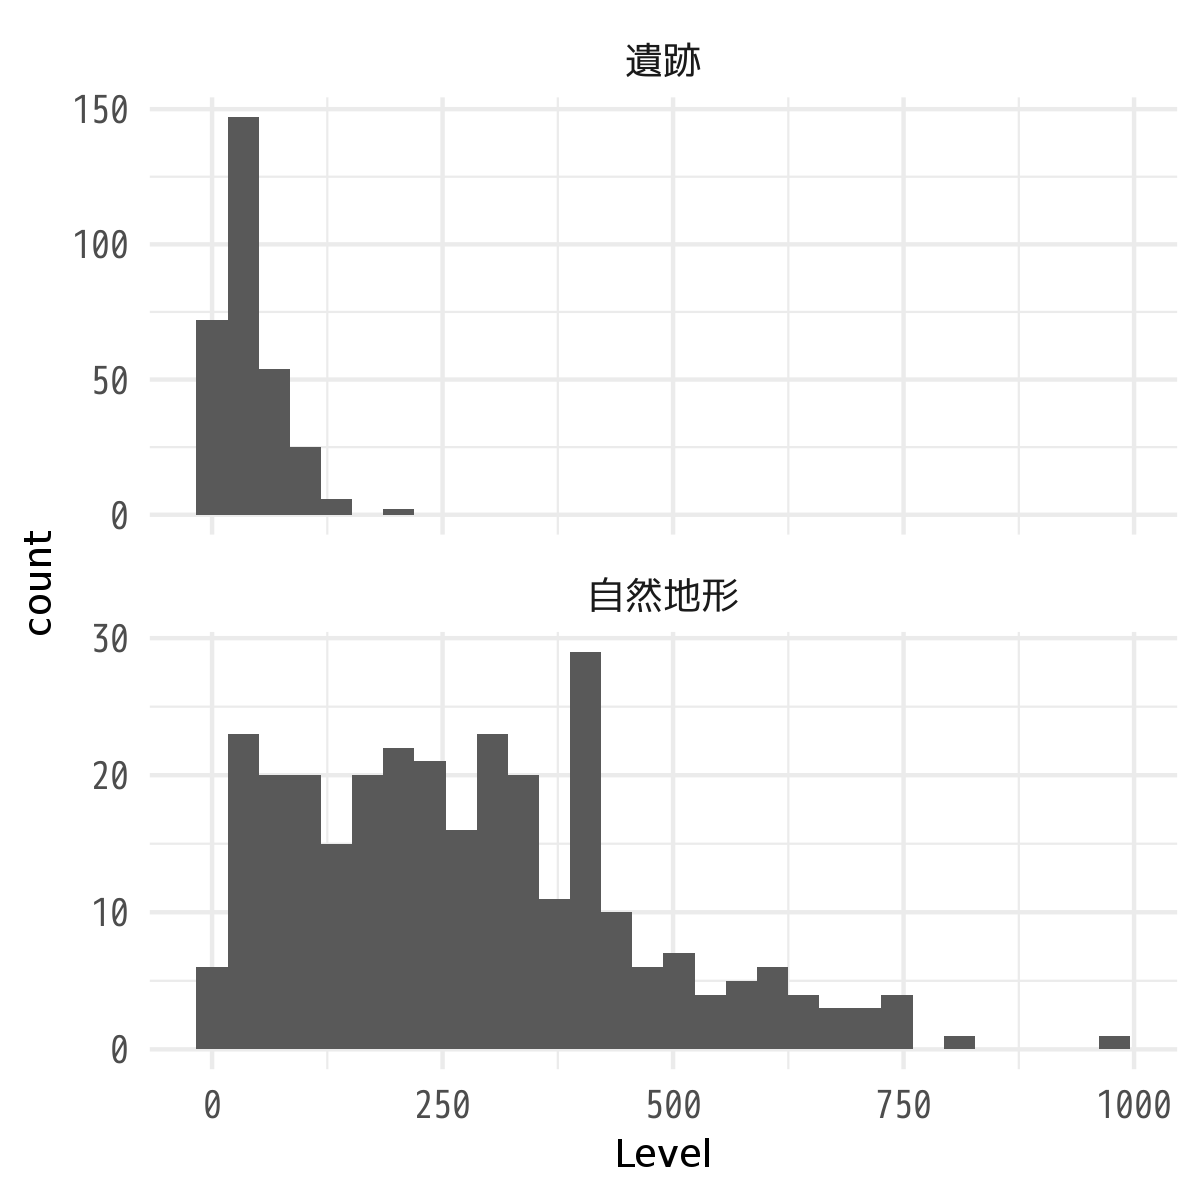
\includegraphics[width=1\linewidth]{R_graph/graph07.png}
\caption{標高}
\end{figurehere}

\begin{figurehere}
\centering
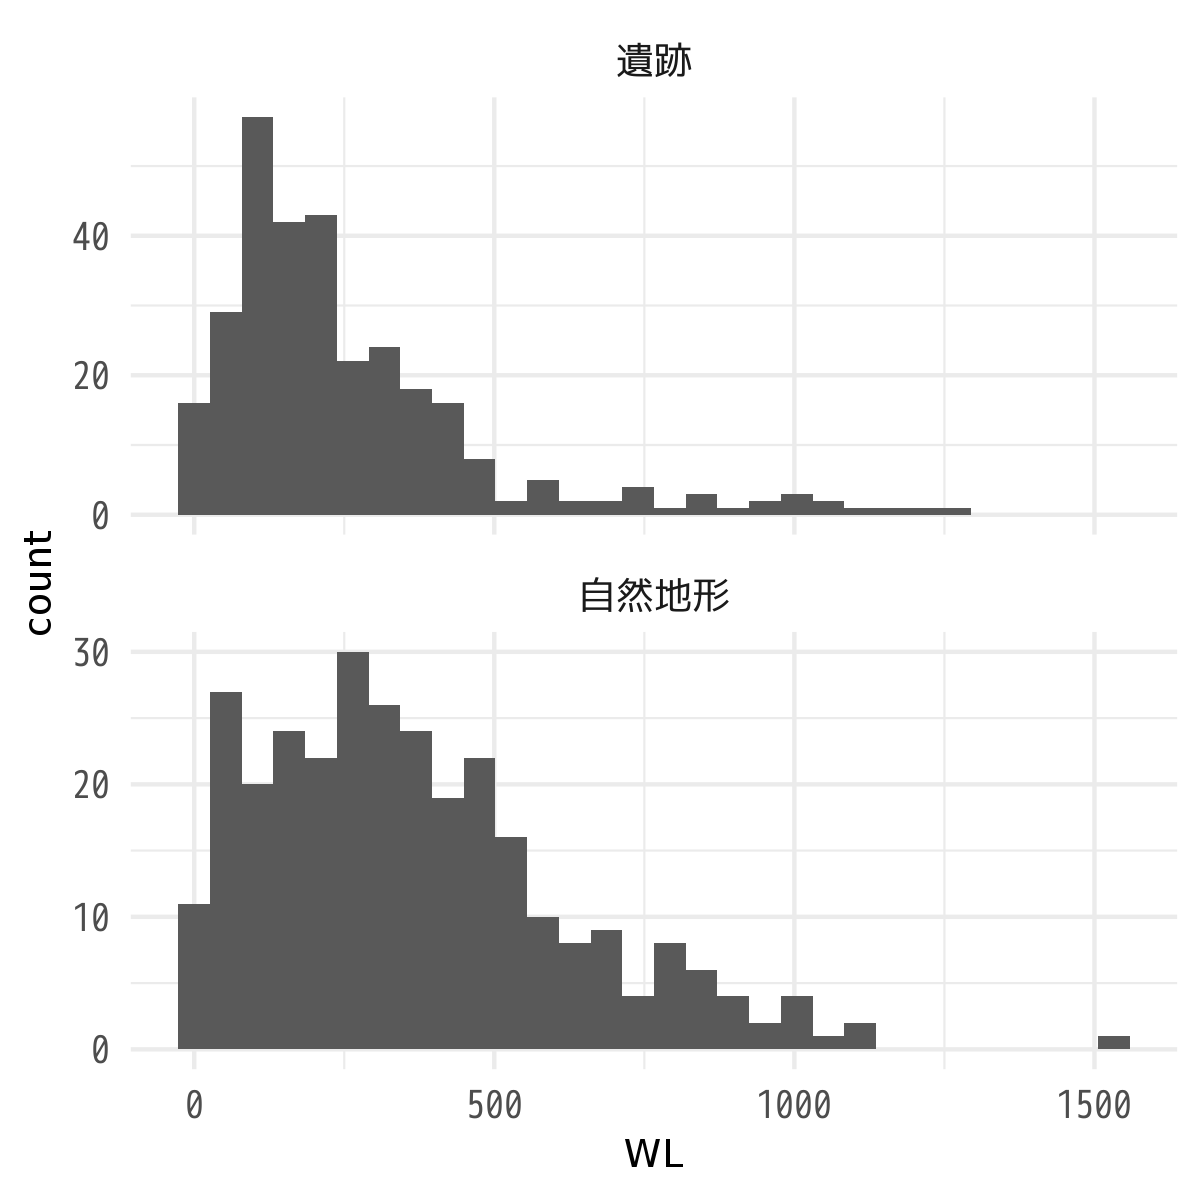
\includegraphics[width=1\linewidth]{R_graph/graph08.png}
\caption{河川からの距離}
\end{figurehere}

\begin{figurehere}
\centering
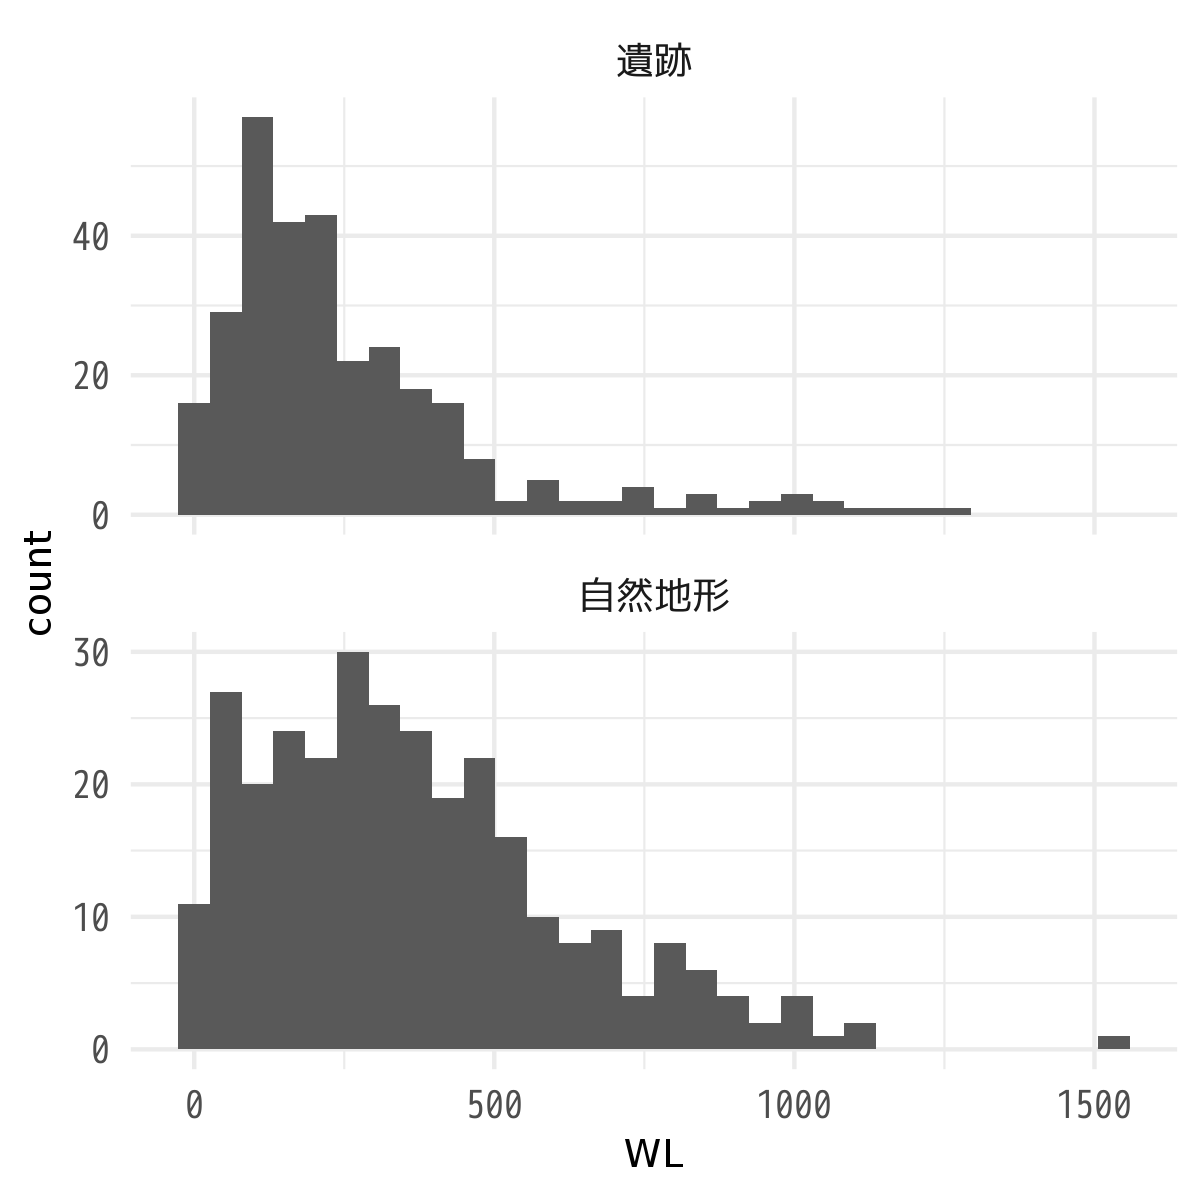
\includegraphics[width=1\linewidth]{R_graph/graph08.png}
\caption{斜面方位}
\end{figurehere}

%%%%
\section{GISと統計処理}
GISは地理データの統計処理を行うためには不可欠の道具です。ただし、GISが統計を行ってくれるわけではありません。多くの場合、統計処理を行う場合はGISからデータを出力して別のソフトウェアで行います。

こうした統計的な用途には、意外にも表計算ソフト不向きです。ヒストグラムは小学校で習う基本的なグラフですが、エクセルでこれをつくるのは案外面倒なものです。本研修では統計処理について深くは触れませんが、地理データから情報を引き出すためには統計処理も大切な技術となります。

%%%%
\section{GISをマスターするために}
GISをマスターするためには実際に手を動かしてソフトウェアを使うことです。「地図の入る書類は何でもQGISでつくる」というほどの意気込みで取り組んでみてください。QGISに「できないことはない」と信じることも重要です。できないのではなく「できることを知らないだけ」ということがほとんどです。

%%%%
\section{GISと発掘データ}
私たち埋蔵文化財行政にかかわる者は何を「記録」として残すべきでしょうか。記録や観察の成果として私たちは「実測図」にこだわります。発掘調査成果の多くはトレーニングを積んだ技師によって描かれた秀麗な「実測図」=「絵」として公開されます。

「絵」を公開することが調査担当者の役割なのか、絵を生成するためのデータを公開することが調査担当者の役割なのか、そうしたことを真剣に議論する時期に来ているように感じています。「記録保存」の「保存」とは何か、「調査成果」の「活用」とは何か、という議論が必要です

%%%%
\section{データファーストの発想}
今回使用した地形データは「絵」として提供されているわけではありません。色も形もない「データ」として提供されたものを私たちは考古学の調査や研究のツールとして活用しました。

考古学の「実測図」=「絵」への強すぎるこだわりは、誰もが考古学にアクセスできる環境の形成を阻害する危険があります。行政実務としての埋蔵文化財保護行政と考古学を同一視しないこと、その結果として「絵」を埋蔵文化財保護行政の評価基準にしないことが必要なのではないでしょうか。

%\end{multicols}
\end{document}
